%!TEX root = ../swiatlow_thesis.tex
\label{appendix:qjets}

\section{Introduction}

\subsection{Overview}
\label{app:qjets:intro:overview}

In some sense, sequential recombination clustering algorithms, such as the \kt-family~\cite{Ellis:1993tq} used by ATLAS and CMS, can be thought of as `undoing' the effects of the parton shower. This somewhat naive view imagines that the tree-like $1\rightarrow2$ splittings of the parton shower have an inverse in the $2\rightarrow1$ mergings of the \textit{clustering history} of a jet. This view is limited, however, by the fact that the parton shower is formally non-invertible: due to the quantum mechanical nature of the splittings, there are many different possible intermediate showering trees which can produce a given set of final state particles. The art of jet algorithms lies in attempting to approximate a reasonable inverse which can reconstruct the initial colored particle which initiated the jet.

A new approach, referred to as Q-jets~\cite{Ellis:2012sn}, admits that there is no unique inverse, and instead allows jets to have many different clustering histories. A normal jet, clustered with the \antikt algorithm, is re-clustered many times using an alternative algorithm which introduces a random element into clustering, thus guaranteeing a distribution of outcomes which can be thought of as corresponding the set of possible parton showers which created the jet. The distribution of clustering histories can be analyzed for each jet, and observables can be constructed based on the properties of the distributions. These observables are found to be able to discriminate between jets initiated by massive boosted objects (such as $W$-bosons) and jets initiated by light quarks or gluons.

This appendix describes a series of studies, published in the ATLAS note~\cite{ATLAS-CONF-2013-087}, which performed the first studies of the Q-jets technique in fully simulated simulation and data\footnote{I gratefully acknowledge the assistance of my co-analyzer and co-editor Lynn Marx, from the University of Washington.}. The ultimate goal was to compare the performance of Q-jets as a boosted object discriminator, especially compared to existing techniques such as n-subjetttiness~\cite{nsub}. Section~\ref{app:qjets:intro:algorithm} gives a brief review of jet clustering and pruning algorithms in general and describes the Q-jets algorithm; the experimental setup as well as the data and Monte Carlo (MC) samples used in this study are presented in Sections~\ref{app:qjets:datasets}; Section~\ref{app:qjets:event-selection} lists the selection criteria for the reconstructed physics objects and the events; the performance of Q-jets in fully reconstructed, simulated events as well as in data is reported in Section~\ref{app:qjets:jetvol}.


\section{The Q-jets algorithm}
\label{app:qjets:intro:algorithm}

Section~\ref{chapter:jets-and-substructure:sequential} introduced the \kt family of clustering algorithms; they are defined by the distance metrics $d_{ij}$ and $d_{iB}$, the exponent $p$, and jet radius parameter $R$. The Q-jets algorithm starts with a typical antikt jet of large enough size to potentially contain a boosted $W$-boson (in these studies, $R=0.7$). 

Further modifications of the jet are possible using jet grooming algorithms to achieve potential improved robustness against pile-up, mass resolution, etc.~\cite{Krohn:2009th,Ellis:2009me,pruning2009}, as discussed in Section~\ref{chapter:jets-and-substructure:grooming}. The \emph{pruning} procedure\cite{Ellis:2009me} is one such example, and plays an important role in the formulation of Q-jets. Pruning proceeds as follows:
%
\begin{enumerate}
      \item Start with a jet found by any jet algorithm and collect its constituents into a list. In this study, $R=0.7$ anti-$k_t$ jets are used.%Define parameters $d_{cut}$ and $z_{cut}$.
      \item Re-run a jet algorithm\footnote{Possible algorithms are $k_t$ and C/A to ensure a meaningful clustering history.} on the list of constituents, checking for the following conditions in each $(i,j) \to p$ recombination;
      \begin{equation}
        z_{ij}=\frac{\min(p_{{\rm T},i}, p_{{\rm T},j})}{|\vec{p_{{\rm T},i}}+\vec{p_{{\rm T},j}}|}<z_{\rm cut}~\mathrm{and}~\Delta R_{ij} > d_{\rm cut}.
         \label{eqn:pruning:cuts}
      \end{equation}
      \item If both the conditions in the previous step are met, discard the softer of the two branches $i$ or $j$ from the jet.
      \item The resulting jet is the \emph{pruned jet}, and can be compared with the jet found in step 1.
\end{enumerate}
%
Both ATLAS and CMS have extensively studied this algorithm; ATLAS has in general preferred the trimming procedure, while CMS has used pruning in several analyses~\cite{ATLAS-SS-2011,Aad:2015fna,Khachatryan:2014gha}.

The Q-jets algorithm is an extension of the pruning procedure. The key to the procedure is the rejection of merges which fail the $z_{\rm cut}$ and $d_{\rm cut}$: if the pairings are somewhat randomized, then the rejection procedure will throw out different branches each time and result in a different final jet. The main difference lies in the distance metric used to determine the order of merging. The algorithm proceeds as follows:
%
\begin{enumerate}
   \item Start with a jet found by any jet algorithm and collect the constituents into a list. 
   \item Compute a set of weights $\omega_{ij}$, which reflect how likely a pair of four-vectors is to be merged, for all pairs of four-vectors. Here, the weights are chosen to be defined as:
   %
\begin{equation}
\omega^{(\alpha)}_{ij}=\exp{\left\{-\alpha\frac{d_{ij}-d^{\rm min}}{d^{\rm min}}\right\}}
\label{eqn:omega}
\end{equation}
%
where $\alpha$ is the \textit{rigidity} which controls the sensitivity of the pair selection to the random number generation, $d_{ij}\equiv\Delta R^2_{ij}=\Delta y^2_{ij}+\Delta \phi^2_{ij}$ the distance measure for the $(i,j)$ pair and $d^{\rm min}$ the minimum of the distance between all pairs. Then the probability $\Omega_{ij} = \omega_{ij}/N$ is defined, where $N = \sum \omega_{ij}$. 
   \item Instead of finding the single minimum $d_{ij}$ as in Equation~\ref{eqn:clustering}, generate a random number, using Equation~\ref{eqn:omega} as a probability density function, and choose a pair of four-vectors as above according to the probabilities $\Omega_{ij}$.
   \item Consider this pair for merging, and veto (as in normal pruning) if they fail the cuts in Equation~\ref{eqn:pruning:cuts}.
   \item Continue until all pairs are merged: the result is one Q-jet. The algorithm can be repeated multiple times to generate a distribution of Q-jets for every jet.
\end{enumerate}

By definition, the closest pair will have a weight $\omega_{ij} = 1$, while all others will have some weight that is suppressed by both the distance metric and the parameter $\alpha$. As $\alpha\rightarrow\infty$, %the weight of the closest pair remains $1$ while all others become exponentially suppressed, resulting in an overwhelming selection of the closest pair and a restoration 
the behavior becomes equivalent to that of the standard pruning procedure. As $\alpha\rightarrow 0$, all pairs begin to acquire similar weights, and so the selected pair can very often be different from the closest pair. Therefore, unlike in both standard recombination techniques and jet pruning, re-running the Q-jets algorithm on a jet does not guarantee the same result, and indeed, it is precisely this behavior which allows the generation of distributions of Q-jets for every input jet.%\footnote{To maintain reproducibility between subsequent productions of a dataset, the seed for the random number generator is set uniquely and reproducibly for each event.}.

Figure~\ref{fig:Qjet_diagram} diagrammatically demonstrates the Q-jets algorithm. The constituents of a single jet are reclustered many times using the algorithm, as shown in the different columns in the diagram. The final jet, at the end of each iteration, is slightly different because different constituents were discarded in the course of the clustering, and so each final jet has different kinematics, e.g. a different mass.

\begin{figure}[htbp]
\centering
\includegraphics[width=.95\textwidth]{QJetDiagram.pdf}
\caption{Diagrammatic example of several different iterations of the Q-jets algorithm in a simplified one-dimensional space. Lines indicate jet constituents/pseudo-jets, distances between lines indicate spatial ($\Delta R$) distances, and line heights indicate constituent energy. The same jet is reclustered many times, with the clustering history starting at the top and proceeding downwards. At each step of the clustering, a different pair is randomly selected, as described in the text, and the pruning criteria are checked: in the case of a failure, the softer of the pair is discarded. Different iterations of the algorithm are displayed in different columns. Discarded constituents are displayed in light grey; merged constituents in hashed blue.} 
\label{fig:Qjet_diagram}
\end{figure}

Figure~\ref{fig:Qjet_distrib} shows typical examples of the mass distributions of Q-jets for several values of $\alpha$ in simulation for a single jet from a dijet sample and a jet from a $W$ boson decay in a $t\bar{t}$ event. It is clear that the distributions have different shapes, with the distribution from light quark and gluon jets being generally wider. This is related to the mass from light quark and gluon jets being more `random' itself: it arises from the chance soft, wide-angle radiation around a single hard core, and the removal of this soft radiation has a large effect in the mass. In contrast, the mass of the $W$ comes from the hard two-prong structure of the $W$ decay, and is resilient to particles being removed. The number of Q-jets generated per jet, $N_{QJets}$, is a free parameter and was set to 1000 in this example. The $z_{\rm cut}$ and $d_{\rm cut}$ values used are $0.1$ and $m_{\rm jet}/p_{\rm T, jet}$, respectively.

\begin{figure}[htbp]
\centering
\subfigure[]{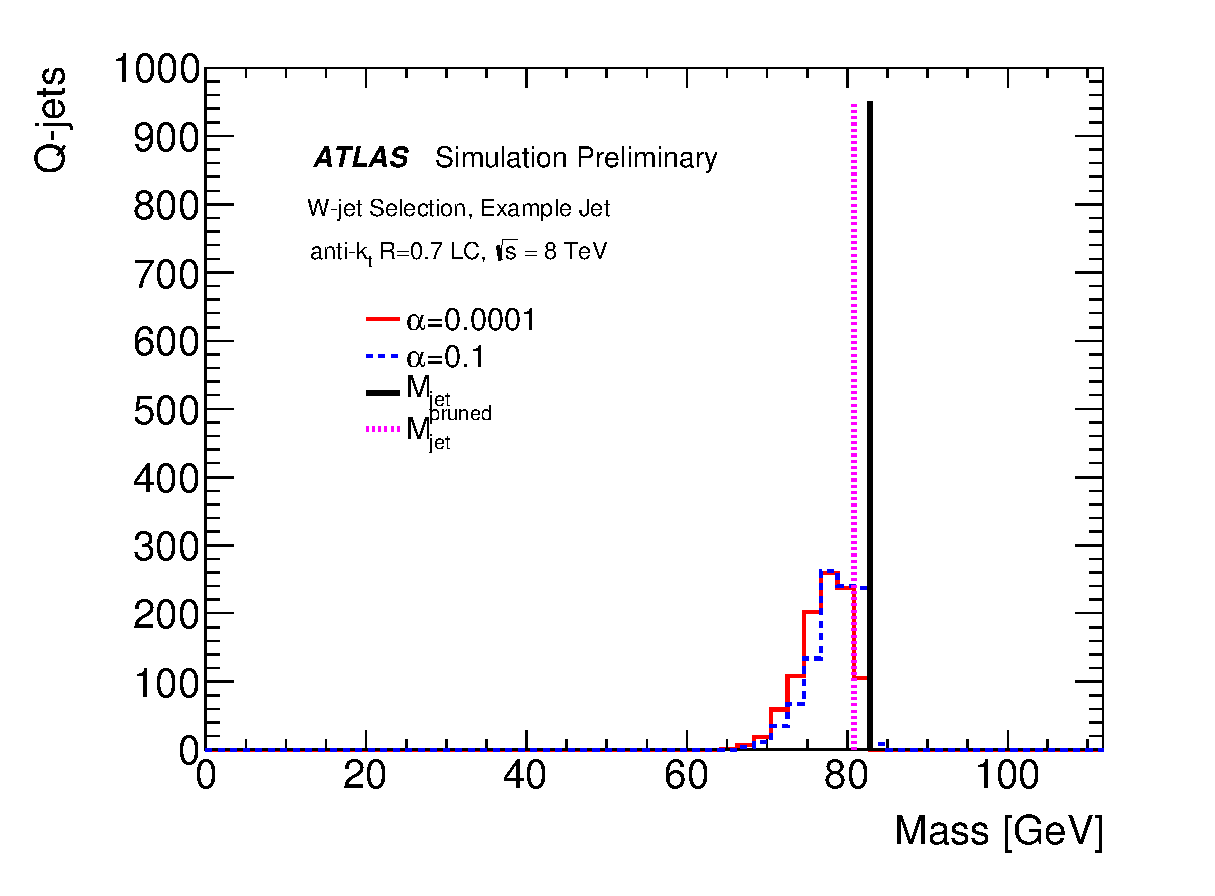
\includegraphics[width=.49\textwidth]{Wjetmass.eps}}
\subfigure[]{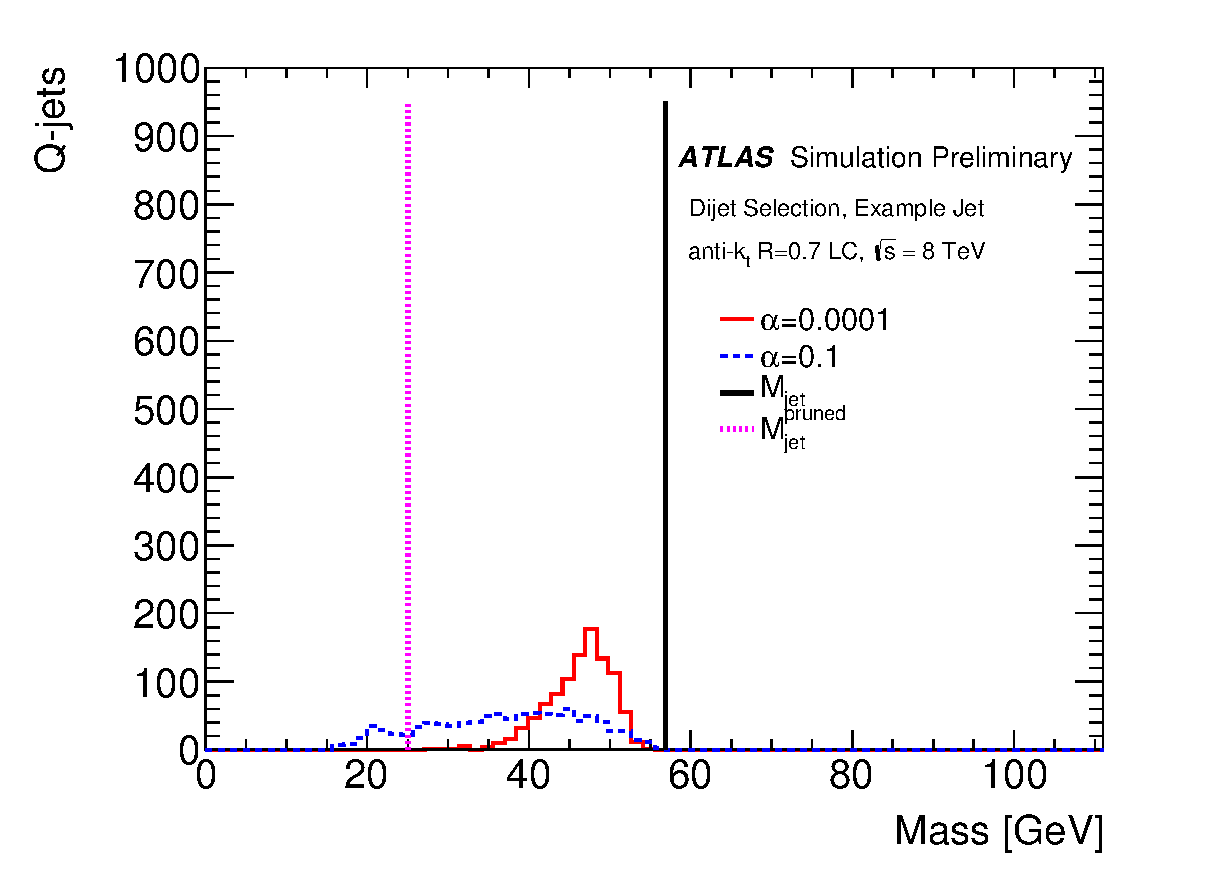
\includegraphics[width=.49\textwidth]{QCDjetmass.eps}}
\caption{Q-jet mass distribution when generating 1000 Q-jets per jet for (a) a jet from a $W$ boson decay in a $t\bar{t}$ event and for (b) a jet from a dijet event, reconstructed from topological clusters. The distribution for $\alpha=100$ is not shown as it coincides with the pruned jet mass, as expected.} %{\bf [*** Remake this plot to fix labels, maybe choose other events]}}
\label{fig:Qjet_distrib}
\end{figure}

\section{Dataset}
\label{app:qjets:datasets}

As with the other 8 TeV studies in this thesis, the full $(20.3\pm0.6)$\invfb of integrated luminosity~\cite{ATLASLumi} is used in the analysis. Two different data samples are used for the studies. The first is similar to the $t\bar{t}$ selection of Chapter~\ref{chapter:color}, but uses only the muon channel for simplicity. A logical OR of a $p_{\rm T}>24$~GeV threshold, isolated muon trigger chain and a $p_{\rm T}>36$~GeV threshold muon trigger chain without the isolation requirement are used to select this sample, which reconstructs semi-leptonic $t\bar{t}$ events and studies the hadronically decaying $W$. The second sample is selected by a single jet trigger chain with a $p_{\rm T}>145$~GeV threshold for anti-$k_t$ $R=0.4$ jets. This trigger is used to select events where the trigger jet $p_{\rm T}$ is not too dissimilar from the $p_{\rm T}$ region of interest: however, this low threshold in $p_{\rm T}$ leads to a very large trigger rate, and therefore only a small, randomly selected subset of the triggered events are recorded. The luminosity of the dijet data sample is thereby reduced to $36.3\pm0.1$\invpb, which still constitutes a sample large enough for the study.

%\cite{Nason:2004rx,Frixione:2007vw}
%\cite{pythia}
%\cite{pythia8}


The $t\bar{t}$ sample is modeled with the \Powheg generator, which incorporates next-to-leading order (NLO) QCD matrix elements into a parton shower framework through the \Pythia simulation, as in Chapter~\ref{chapter:color}. The light quark and gluon background sample is modelled with dijet samples produced with the \Pythia generator. 


\section{Event Selection}
\label{app:qjets:event-selection}

\subsection{$W$-jet selection}

A sample enriched in boosted hadronically-decaying $W$ bosons is chosen from events that have passed a selection for $t\bar{t}\to WbWb$ events, where one $W$ boson decays leptonically into a muon and a neutrino, and the other decays hadronically. A standard pre-selection of quality cuts is applied to all events. Events with exactly zero good electron candidates and one good muon candidate, which has to be matched to a muon trigger object, are required. At least four good anti-$k_t$ $R=0.4$ jets need to be reconstructed in the event, out of which at least one is required to be $b$-tagged at the $70\%$ operating point of the MV1 algorithm. The missing transverse energy \Etmiss in the event must be larger than 20~GeV and the sum of the $E_{\rm T}^{miss}$ and the transverse mass of the leptonically-decaying $W$ boson, reconstructed by combining the muon candidate and the \Etmiss, must be larger than 60~GeV. The highest $p_{\rm T}$ anti-$k_t$ $R=0.7$ jet must have $|\eta|<1.8$, to ensure that it is contained in the tracking volume. The same jet must not overlap with a selected $b$-tagged jet and is required to have a pruned mass of $50<m_{\rm jet}^{\rm pruned}<110$~GeV and $200<p_{\rm T}<350$~GeV. 



\subsection{Dijet selection}


After applying the preselection criteria (consisting of standard quality cuts), the sub-leading anti-$k_t$ $R=0.7$ jet is considered and required to have a pruned mass of $50<m_{\rm jet}^{\rm pruned}<110$~GeV and $200<p_{\rm T}<350$~GeV. The leading anti-$k_t$ $R=0.4$ jet is required to pass the single jet trigger described in section~\ref{app:qjets:datasets} and have $p_T > 180$~GeV in order to lie on the fully efficient region of the trigger turn-on curve. Furthermore, to reduce biases introduced by the trigger selection, the leading anti-$k_t$ $R=0.4$ jet is required to be isolated from the second highest $p_{\rm T}$ anti-$k_t$ $R=0.7$ jet with $\Delta \phi > 2.0$ to guarantee that no part of the jet which fired the trigger overlaps with the jet under study.

\section{Jet Volatility}
\label{app:qjets:jetvol}

\subsection{Overview}
\label{app:qjets:jetvol:overview}

As previously discussed, the main power of Q-jets as a jet tagger comes from the relative stability of the mass distribution for $W$-bosons compared to light quark and gluon jets. This stability is related to the origin of the mass of the $W$-jet in its two-prong structure, compared to the soft, wide-angle radiation causing the mass in light quark and gluon jets. One way to capture these different outcomes is to define the \textit{volatility}:
%
\begin{equation}
\nu=\Gamma/\langle m \rangle
\end{equation}
%
where $\Gamma=\sqrt{\langle m^2 \rangle-\langle m \rangle^2}$ and $\langle m \rangle$ are the RMS deviation and the mean of the Q-jets jet mass distributions, respectively.

Figure~\ref{fig:Vollog} shows the separation in the volatility between $W$-jets from the $t\bar{t}$ sample and light quark and gluon jets. The latter have a much larger volatility, as expected: the variation is much larger when running the Q-jets procedure, as the source of the light quark and gluon mass is less table. Truth jets, which are constructed from truth particles taken from the MC event record shown in Figure~\ref{fig:TruthVollog}, have slightly lower volatility than jets reconstructed from topological clusters, as shown in Figure~\ref{fig:RecoVollog}. As truth jets do not have any pileup in them, they are expected to have a slightly lower variation. For both of these figures, a rigidity of $\alpha = 0.1$ and a $N_{Q-jets} = 75$ was used.


\begin{figure}[htbp]
\centering
\subfigure[Truth Jets \label{fig:TruthVollog}]{\includegraphics[width=.45\textwidth]{NoGroomedBOverlapWithMassCutAntiKt7Truth_lj_MassVolatility_PT200_eta0_logy_.eps}}
\subfigure[Reconstructed Jets \label{fig:RecoVollog}]{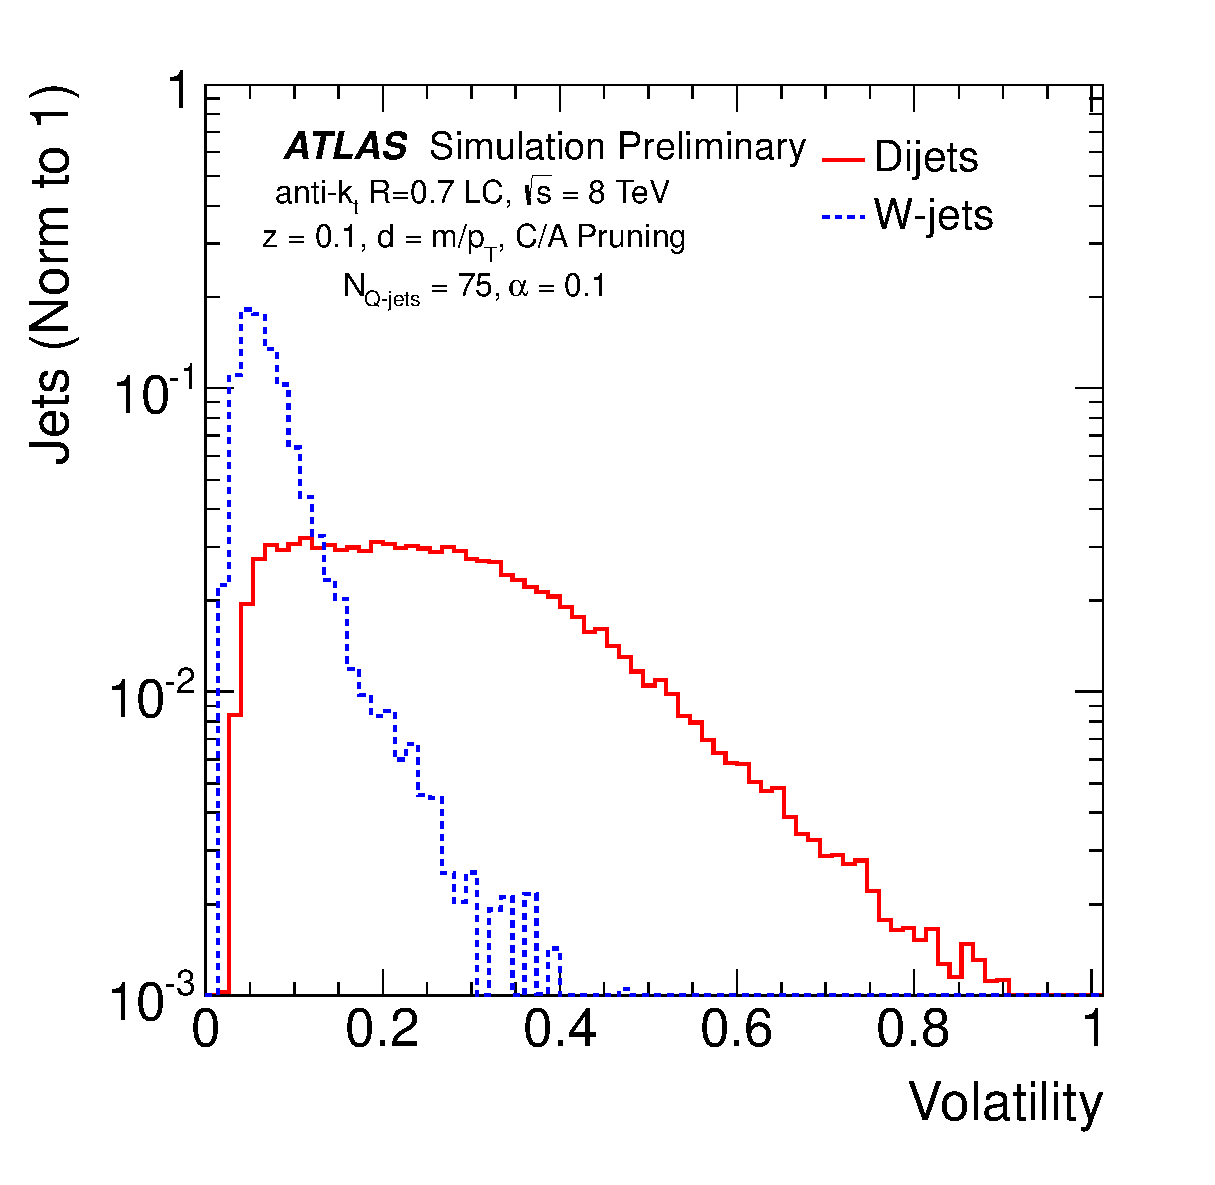
\includegraphics[width=.45\textwidth]{NoGroomedBOverlapWithMassCutAntiKt7LCTopo_lj_MassVolatility_PT200_eta0Log.eps}}
\caption{The volatility distributions for $\alpha = 0.1$ and 75 Q-jets per jet, of $W$-jets compared to dijets for (a) truth-particle jets and for (b) jets reconstructed from locally calibrated topological clusters.} %{\bf [*** Make this also with \boldmath{$\alpha=0.01$} and log axes to compare to theory paper?]}}
\label{fig:Vollog}
\end{figure}

%----------------------------------------------------
% Optimization vs. \alpha
%----------------------------------------------------
\subsection{Optimization vs. $\alpha$}
\label{app:qjets:jetvol:alpha}

As noted in Section~\ref{app:qjets:intro:algorithm}, the volatility variable is expected to depend on the rigidity, $\alpha$. In particular, as $\alpha\rightarrow\infty$, the random element of Q-jets is lost, and the power of volatility decreases. Likewise, as $\alpha\rightarrow 0$, the weighting by the distance metric loses importance, and the selection of mergings becomes completely random and a reduction of separation is again expected. For this reason, a particular value of $\alpha$ is expected to show the best separation between $W$ jets and light quark and gluon jets: just enough randomness is introduced that the light quark and gluon jets lose their stability, but not enough randomness is introduced that the $W$-jet loses its stability.

Figure~\ref{fig:Vol_vs_alpha} shows the mean of the volatility distribution as well as the significance of the volatility as a function of $\alpha$. The significance is defined as the ratio of the absolute difference of the mean $W$-jet selection and dijet selection volatilities to the sum in quadrature of the respective RMS values. It can be seen that the optimal separation occurs at $\alpha = 0.1$. A full comparison of signal efficiency versus background rejection\footnote{The efficiency is defined as the ratio of the number of kept to rejected $W$-jets whereas the rejection is defined as the ratio of the number of rejected to kept light quark and gluon jets.} is presented in Section~\ref{app:qjets:jetvol:rejection}.

\begin{figure}[htbp]
\centering
\subfigure[]{\includegraphics[width=.45\textwidth]{NoGroomedBOverlapAntiKt7LCTopo_lj_MassVolatility_PT200_eta0_mean.eps}}
\subfigure[]{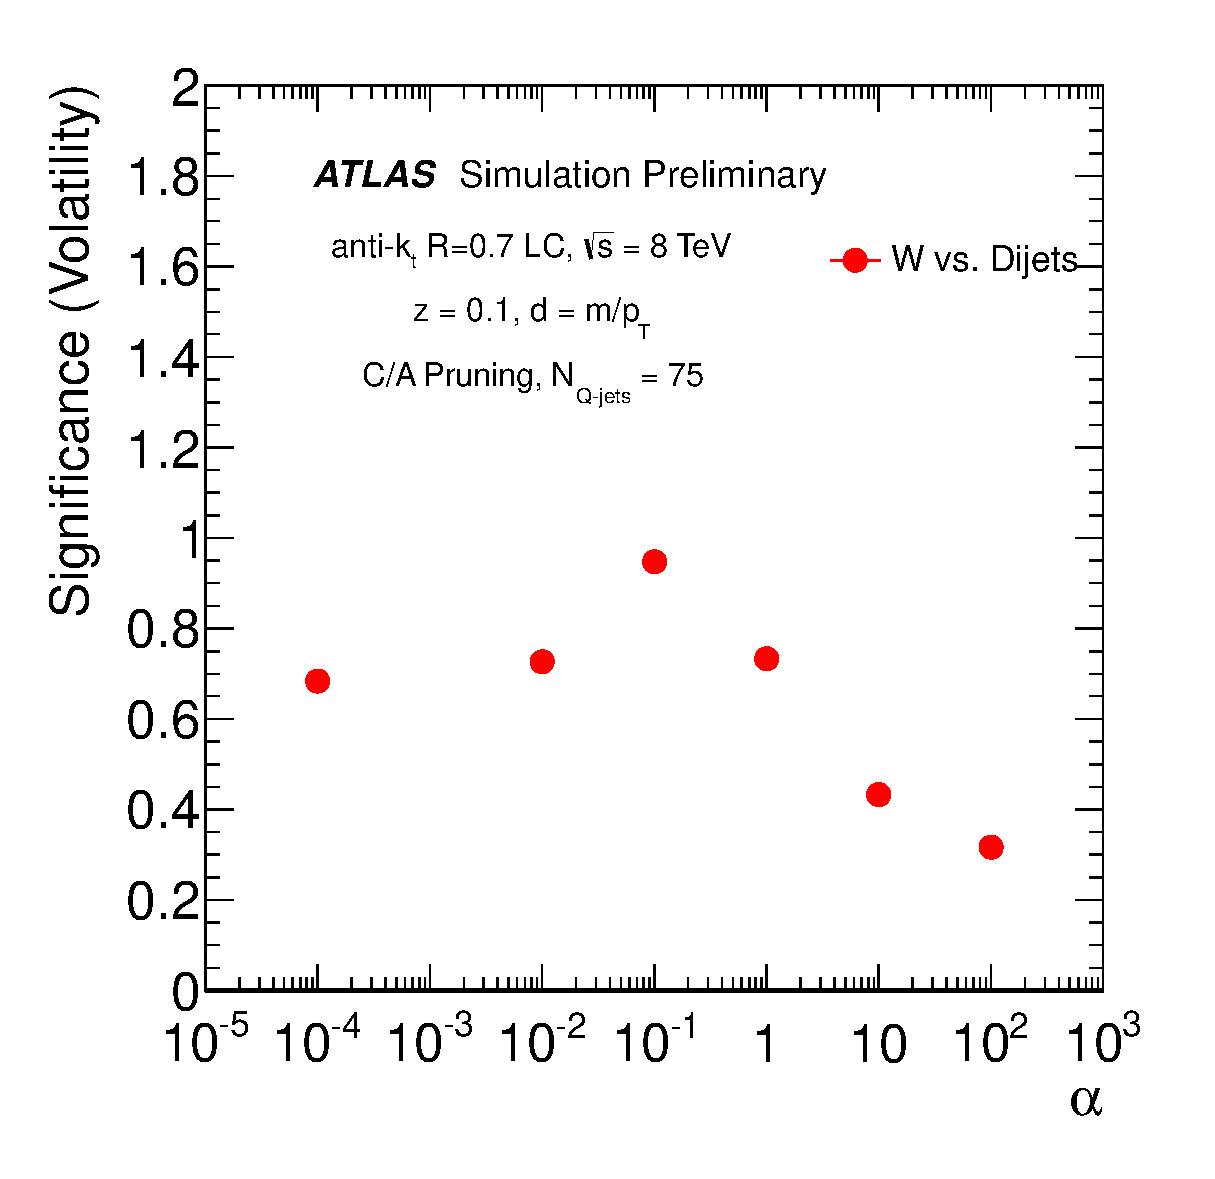
\includegraphics[width=.45\textwidth]{NoGroomedBOverlapAntiKt7LCTopo_lj_MassVolatility_PT200_eta0_meanSig.eps}}
\caption{Distributions of (a) the volatility for $W$-jets and dijets and (b) the significance of the volatility  as a function of the rigidity $\alpha$. The optimal separation in mean and optimal significance is observed at $\alpha = 0.1$. The significance is defined as the ratio of the difference between the mean dijet and mean $W$-jet selection volatilities to the sum in quadrature of the respective RMS values.}
\label{fig:Vol_vs_alpha}
\end{figure}

%----------------------------------------------------
% Optimization of number of QJets, pre-clustering
%----------------------------------------------------
\subsection{Optimization of Q-jet number}
\label{app:qjets:jetvol:number}

Apart from the rigidity $\alpha$, another free parameter of the Q-jets algorithm is $N_{QJets}$, which is the number of Q-jets generated per jet to calculate the volatility. In principle, $\nu$ is defined for $N_{QJets}\to\infty$, but in practice it must be  estimated from finite samples. As $N_{QJets}$ increases, the volatility is expected to become more robust against statistical fluctuations and therefore a stronger discriminant. However, the computation time grows significantly with increasing $N_{QJets}$, which can lead to a heavy load on computing resources. Figure~\ref{fig:Vol_vs_NQJets} displays the mean volatility as a function of $N_{QJets}$. It shows that the separation between $W$-jets and dijets is fairly stable and suggests that analyses are able to use $N_{QJets}$ values a low as $25-50$ to observe similar performance to the results presented in this note, where $N_{QJets}=75$ is generally used. Section~\ref{app:qjets:jetvol:rejection} presents a full signal efficiency versus background rejection optimization for this variable. %(\textit{\textbf{Ed:} We plan on adding a $N_Q = 5$ point as well.})

\begin{figure}[htbp]
\centering
\subfigure[]{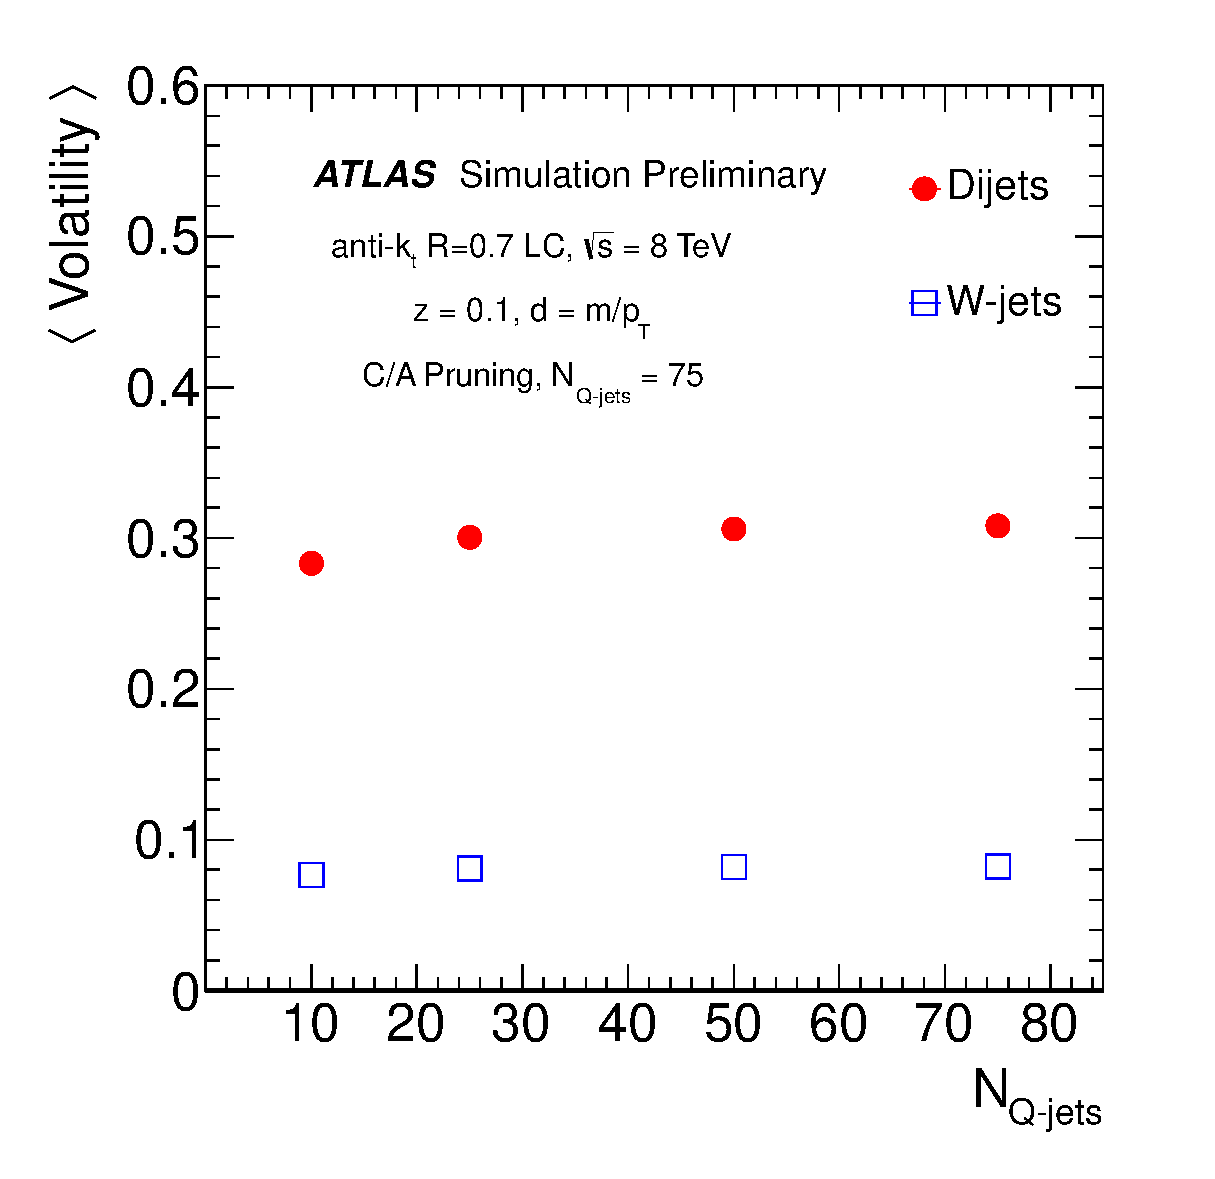
\includegraphics[width=.45\textwidth]{NoGroomedBOverlapAntiKt7LCTopo_lj_MassVolatility_PT200_eta0_meanNQjets.eps}}
\subfigure[]{\includegraphics[width=.45\textwidth]{NoGroomedBOverlapAntiKt7LCTopo_lj_MassVolatility_PT200_eta0_meanNQjetsSig.eps}}
\caption{Distributions of (a) the volatility for $W$-jets and dijets and (b) the significance of the volatility  as a function of $N_{QJets}$. The significance is defined as the ratio of the difference between the mean dijet and mean $W$-jet selection volatilities to the sum in quadrature of the respective RMS values.}% {\bf [*** update with b overlap and fix labels]}}
\label{fig:Vol_vs_NQJets}
\end{figure}

%----------------------------------------------------
% Pileup
%----------------------------------------------------
\subsection{Performance versus pile-up}
\label{app:qjets:jetvol:pileup}

% Volatility shows only a weak dependence on the average number of interactions per bunch crossing for $W$-jets and a negligible dependence for dijets, as shown in Figures~\ref{fig:Vol_vs_MUW} and~\ref{fig:Vol_vs_MUQCD}, respectively. This is in agreement with the expectation that jet pruning works so as to remove pile-up from large $R$ jets~\cite{Ellis2009a,Chatrchyan:2013rla}. The effect is smaller in the dijet sample because pile-up is topologically more similar to dijets than to hadronic decay products of a $W$ boson and therefore has a weaker influence on light quark and gluon jets.
Volatility shows only a small dependence on the average number of interactions per bunch crossing, up to 40, for both $W$-jets and dijets, as shown in Figures~\ref{fig:Vol_vs_MUW} and~\ref{fig:Vol_vs_MUQCD} respectively. As jet pruning is designed partly to remove pileup from large $R$ jets, volatility is likewise expected to have weak sensitivity to pileup, as observed by others~\cite{pruning2009,Khachatryan:2014gha}. 

\begin{figure}[htbp]
\centering
\subfigure[\label{fig:Vol_vs_MUW}]{\includegraphics[width=.44\textwidth]{AntiKt7LCTopo_rig1000_W_MU.eps}}
%\subfigure[\label{fig:Vol_vs_VTXW}]{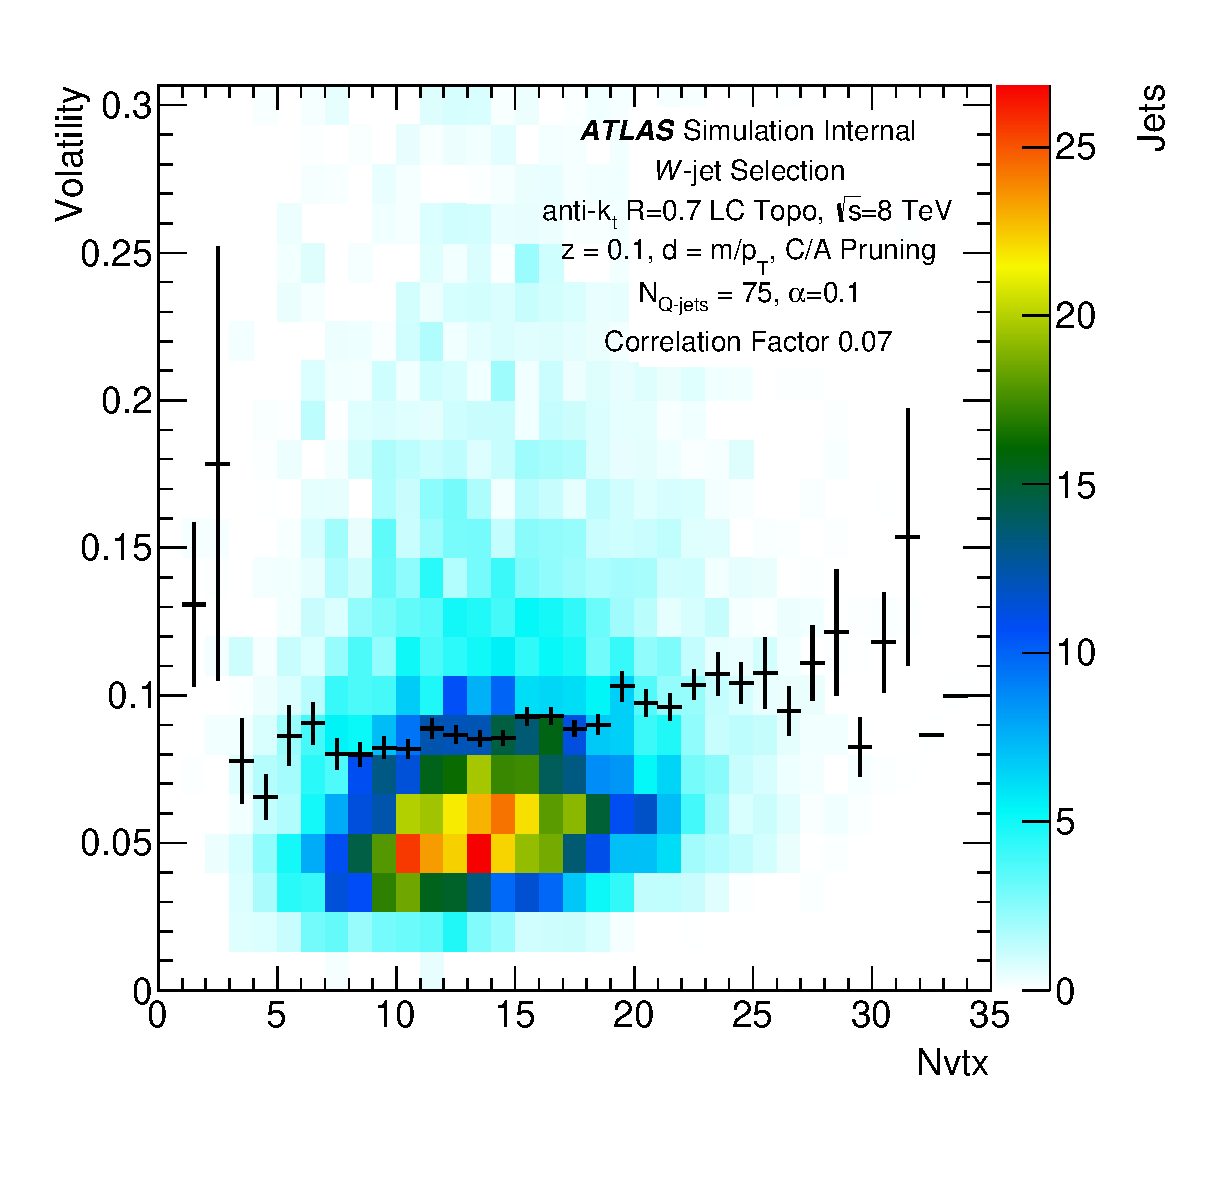
\includegraphics[width=.45\textwidth]{AntiKt7LCTopo_rig1000_W_VTX.eps}}
\subfigure[\label{fig:Vol_vs_MUQCD}]{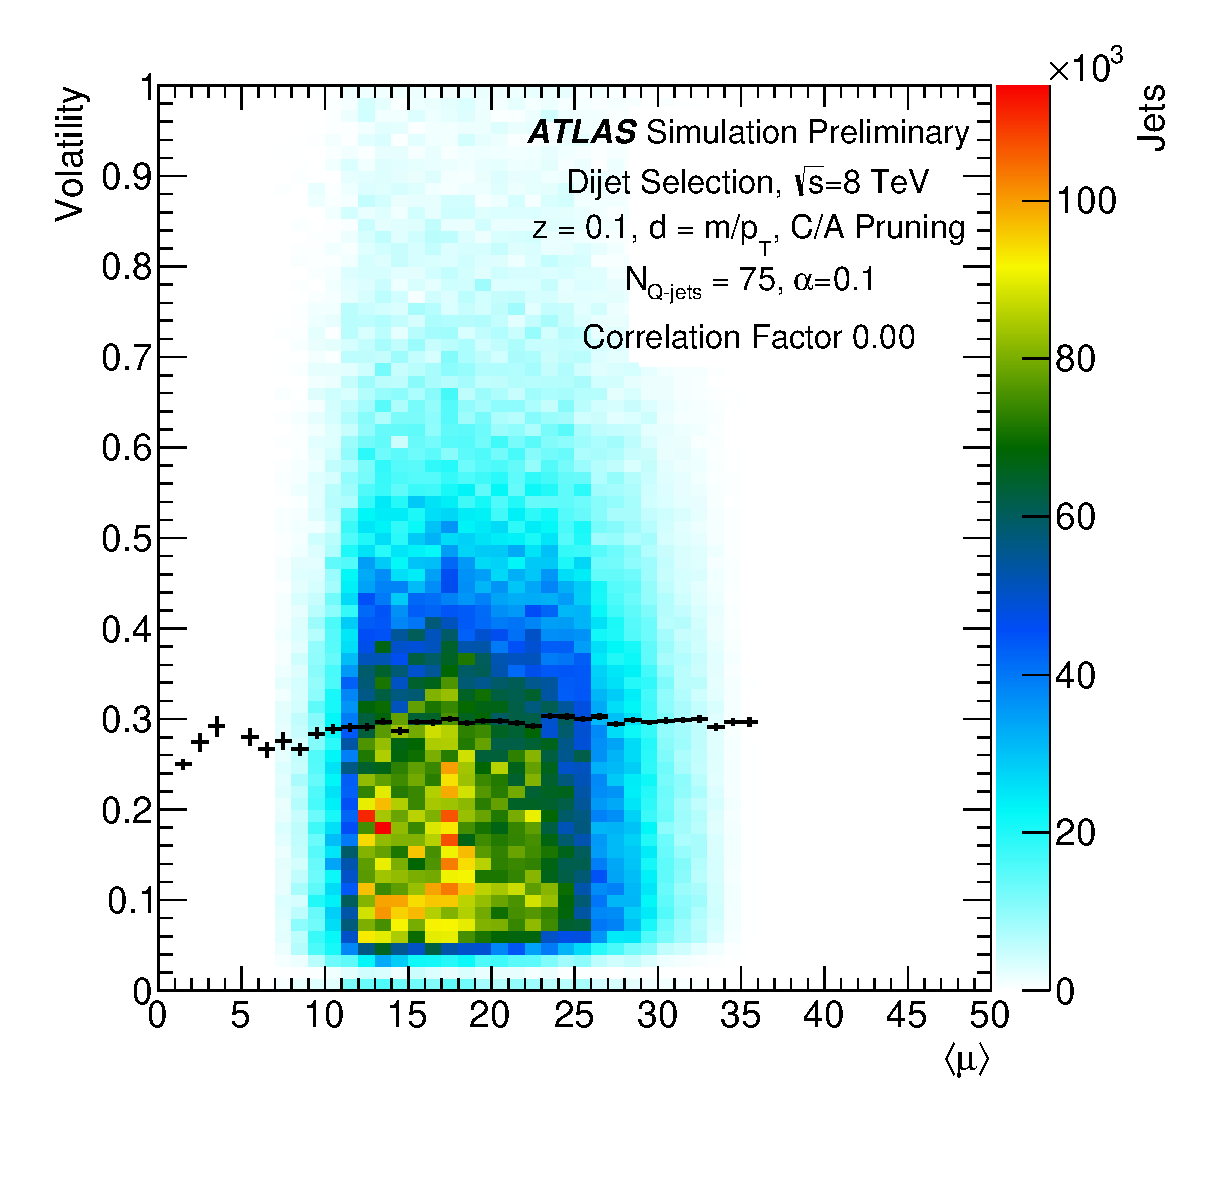
\includegraphics[width=.44\textwidth]{AntiKt7LCTopo_rig1000_QCD_MU.eps}}
%\subfigure[\label{fig:Vol_vs_VTXQCD}]{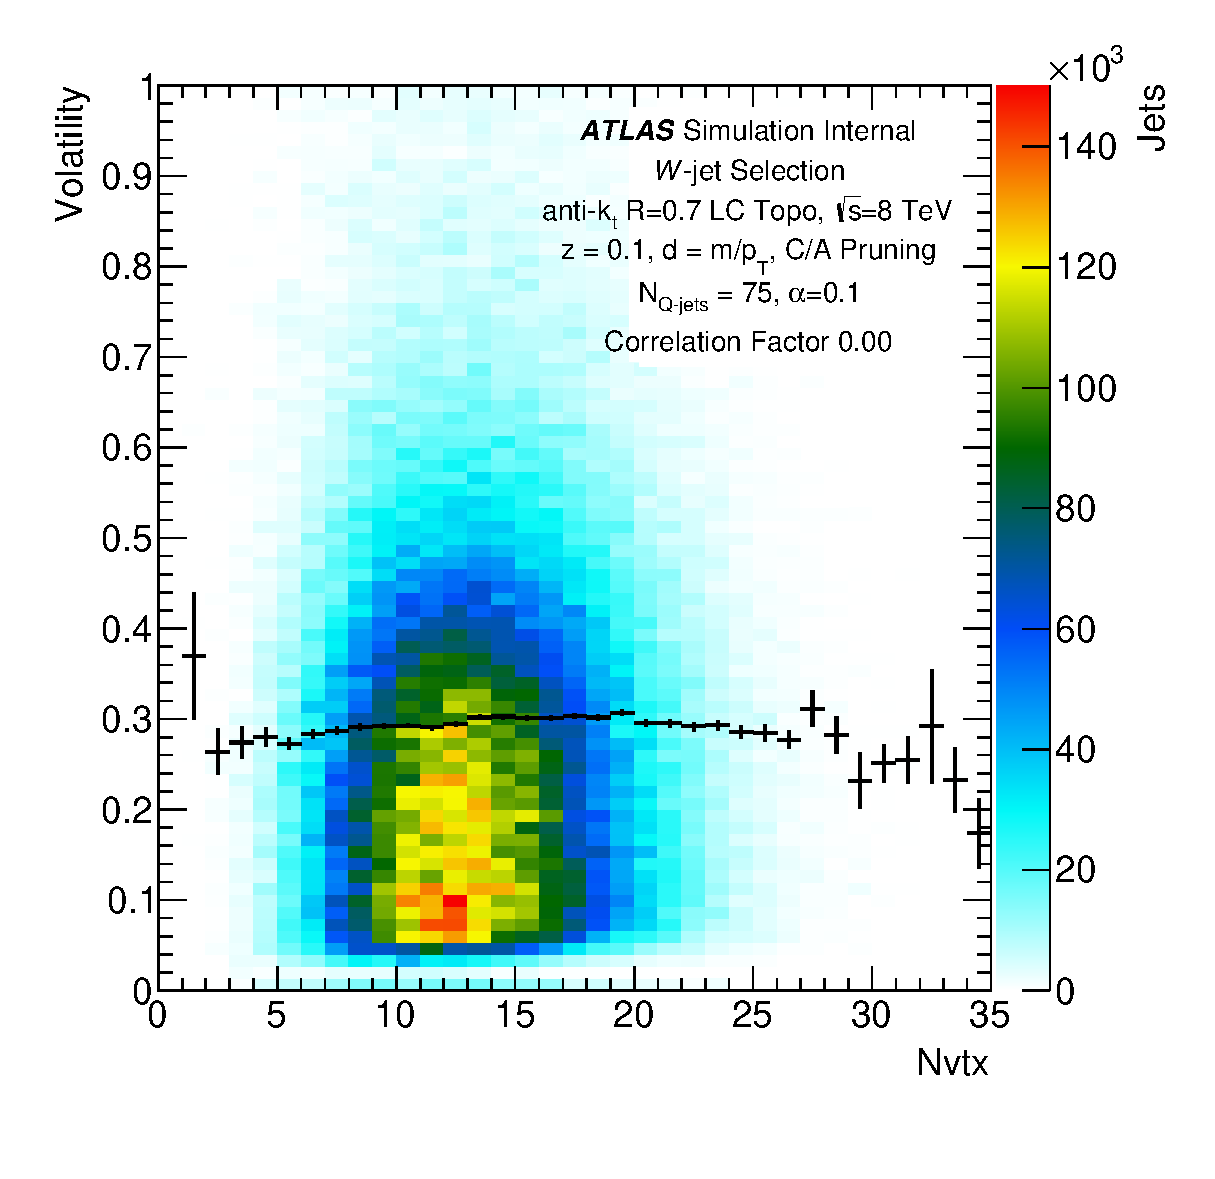
\includegraphics[width=.45\textwidth]{AntiKt7LCTopo_rig1000_QCD_VTX.eps}}
%\caption{Volatility as a function of (left) $\mu$ and (right) number of primary vertices for (top) $W$-jets and (bottom) dijets.}
\caption{Volatility as a function of the average number of interactions per bunch crossing for (a) $W$-jets and (b) dijets for jets reconstructed from topological clusters. The black points represent the mean volatility as a function of $\langle\mu\rangle$.}
\end{figure}

%----------------------------------------------------
% Data/MC comparisons
%----------------------------------------------------
\subsection{Data/MC agreement}
\label{app:qjets:jetvol:datamc}

The comparison of data to MC for the volatility variable is shown in Figure~\ref{fig:DataMC_vol} for an $\alpha$ value of 0.1. Fair agreement is seen in all cases, although in the dijet sample it is generally better and stable over the full range of volatility. In the $W$-jet sample, the Monte Carlo predicts higher values of volatility than seen in data. The comparison of the pruned jet mass distribution in data and simulation in the $W$ mass peak region between 50~GeV and 110~GeV is shown in Figure~\ref{fig:Wpeak}.

\subsubsection*{Systematic uncertainties}

The different sources of systematic uncertainties that are considered can be split into two main categories: those affecting the overall normalization and those affecting the shape of the distributions and the acceptance. For the first category, a 5\% uncertainty on the next-to-next-to-leading order in QCD and next-to-next-to-leading logarithmic order $t\bar{t}$ cross-section~\cite{Aliev:2010zk} is applied as well as a 2.8\% uncertainty on the integrated luminosity. The latter is derived, following the same methodology as that detailed in \cite{ATLASLumi}, from a preliminary calibration of the luminosity scale derived from beam-separation scans performed in November 2012. For the second category, the major sources of uncertainties considered are related to the jet energy scale (JES), jet energy resolution (JER), jet mass scale (JMS) and $b$-tagging efficiency, as described in Chapter~\ref{chapter:jet-reconstruction}. The systematic uncertainties from these different sources are combined and shown in the shaded band in Figures~\ref{fig:DataMC_volW} and~\ref{fig:WpeakW} together with the statistical uncertainty of the simulated samples. Figures~\ref{fig:DataMC_volQCD} and~\ref{fig:WpeakQCD} show statistical uncertainties only.

\begin{figure}[htbp]
\centering
%\subfigure[]{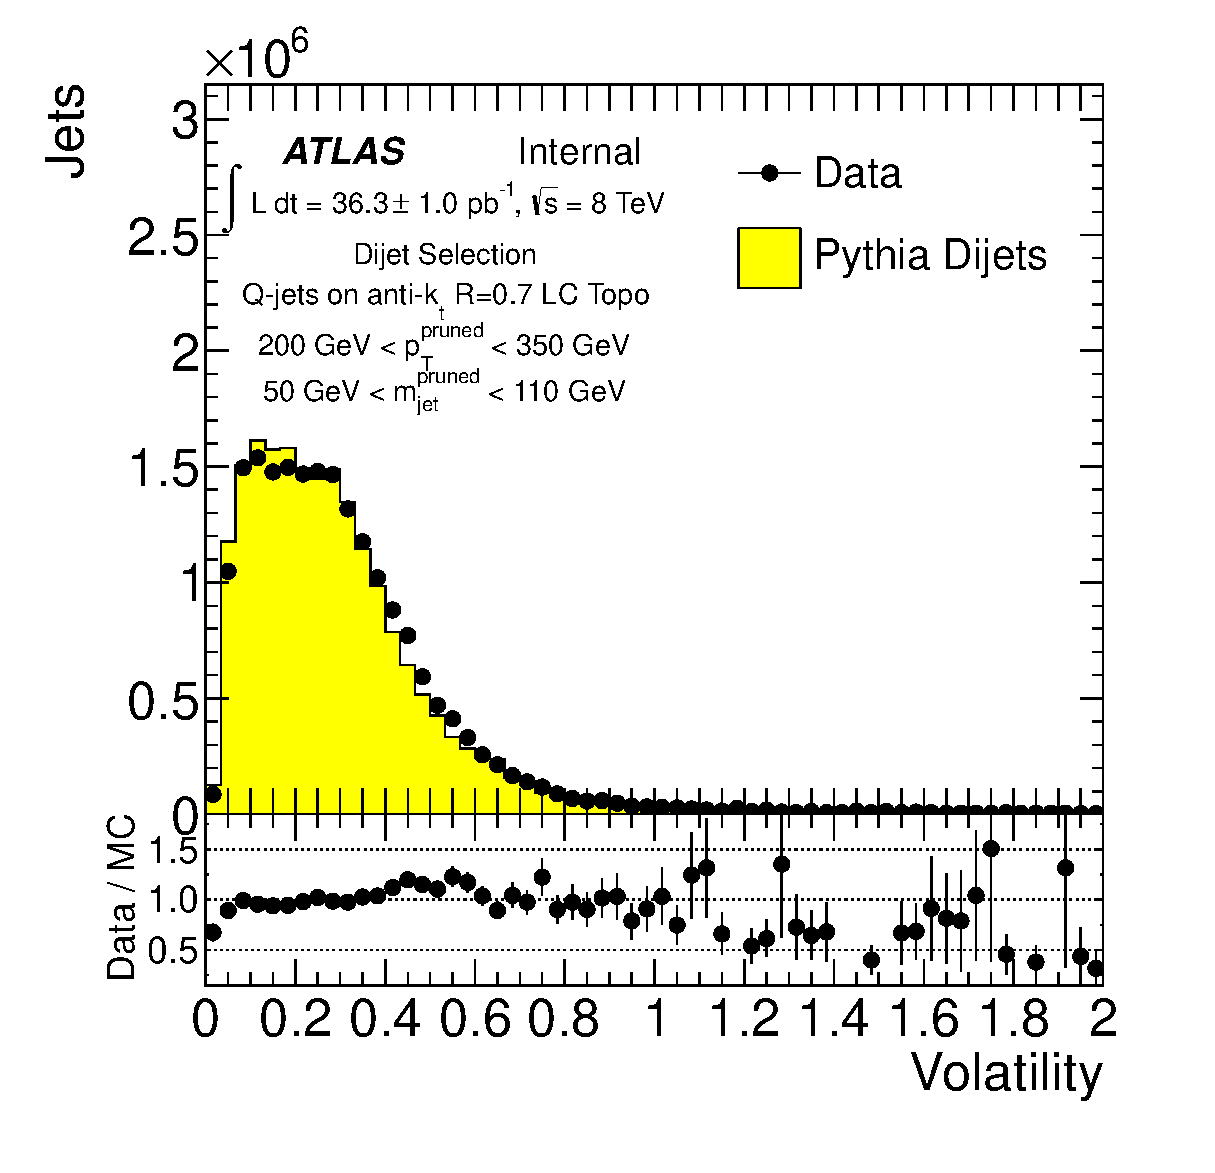
\includegraphics[width=.45\textwidth]{WithMassCutAntiKt7LCTopo_z1_d5_emin0_emax0_rig1000_NJets75_lj_MassVolatility_PT200_eta0_WithData.eps}}
\subfigure[\label{fig:DataMC_volW}]{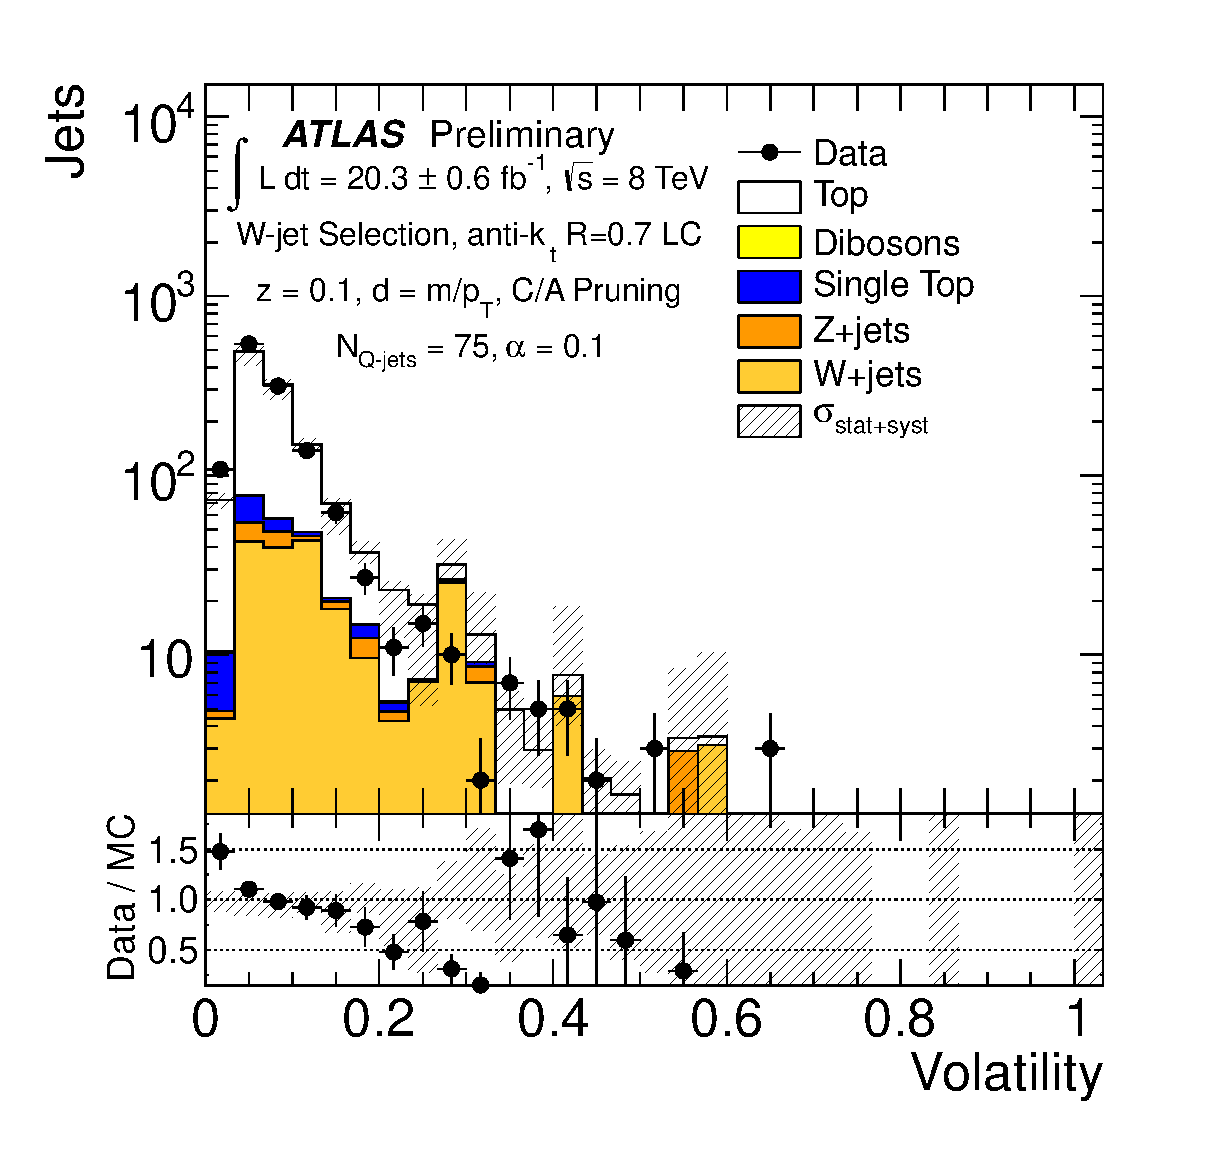
\includegraphics[width=.45\textwidth]{NoGroomedBOverlapWithMassCutAntiKt7LCTopo_z1_d5_emin0_emax0_rig1000_NJets75_lj_MassVolatility_PT200_eta0_WithData_Logy.eps}}
\subfigure[\label{fig:DataMC_volQCD}]{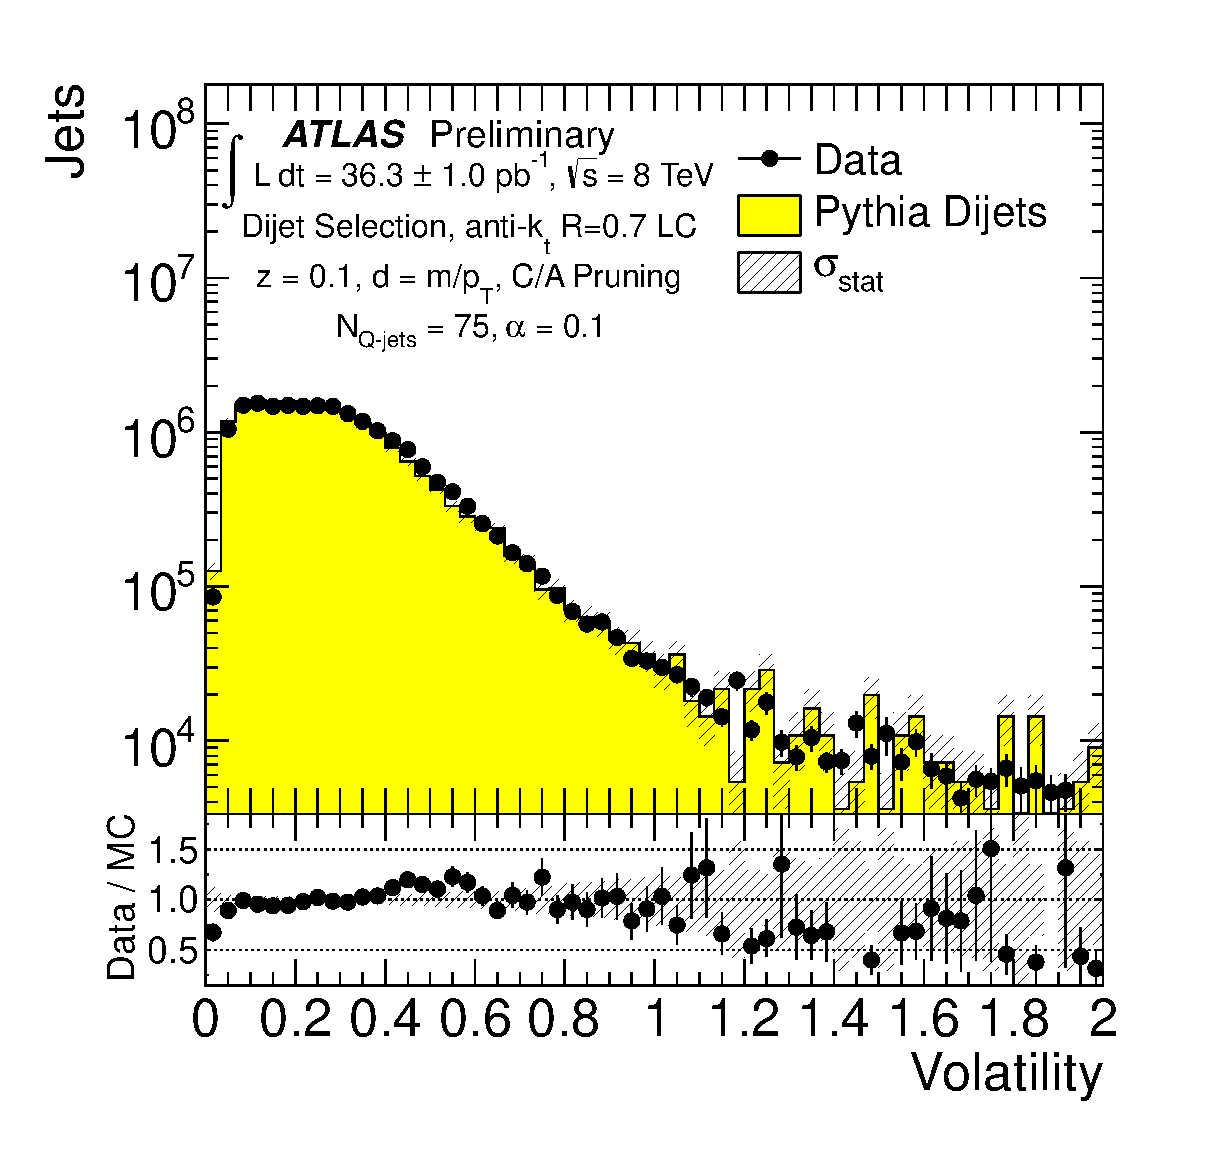
\includegraphics[width=.45\textwidth]{WithMassCutAntiKt7LCTopo_z1_d5_emin0_emax0_rig1000_NJets75_lj_MassVolatility_PT200_eta0_WithData_Logy.eps}}
\caption{Volatility for reconstructed calorimeter jets in data and in simulation for (a) a $W$-jet selection and for (b) a dijet selection. $W$-jet selection plots show statistical and systematic uncertainties whereas dijet selection plots show statistical uncertainties only.}% {\bf [*** fix pT labels, QCD running now, more data (full 21 fb) coming ASAP (next week)]}}
\label{fig:DataMC_vol}
\end{figure}

\begin{figure}[htbp]
\centering
\subfigure[\label{fig:WpeakW}]{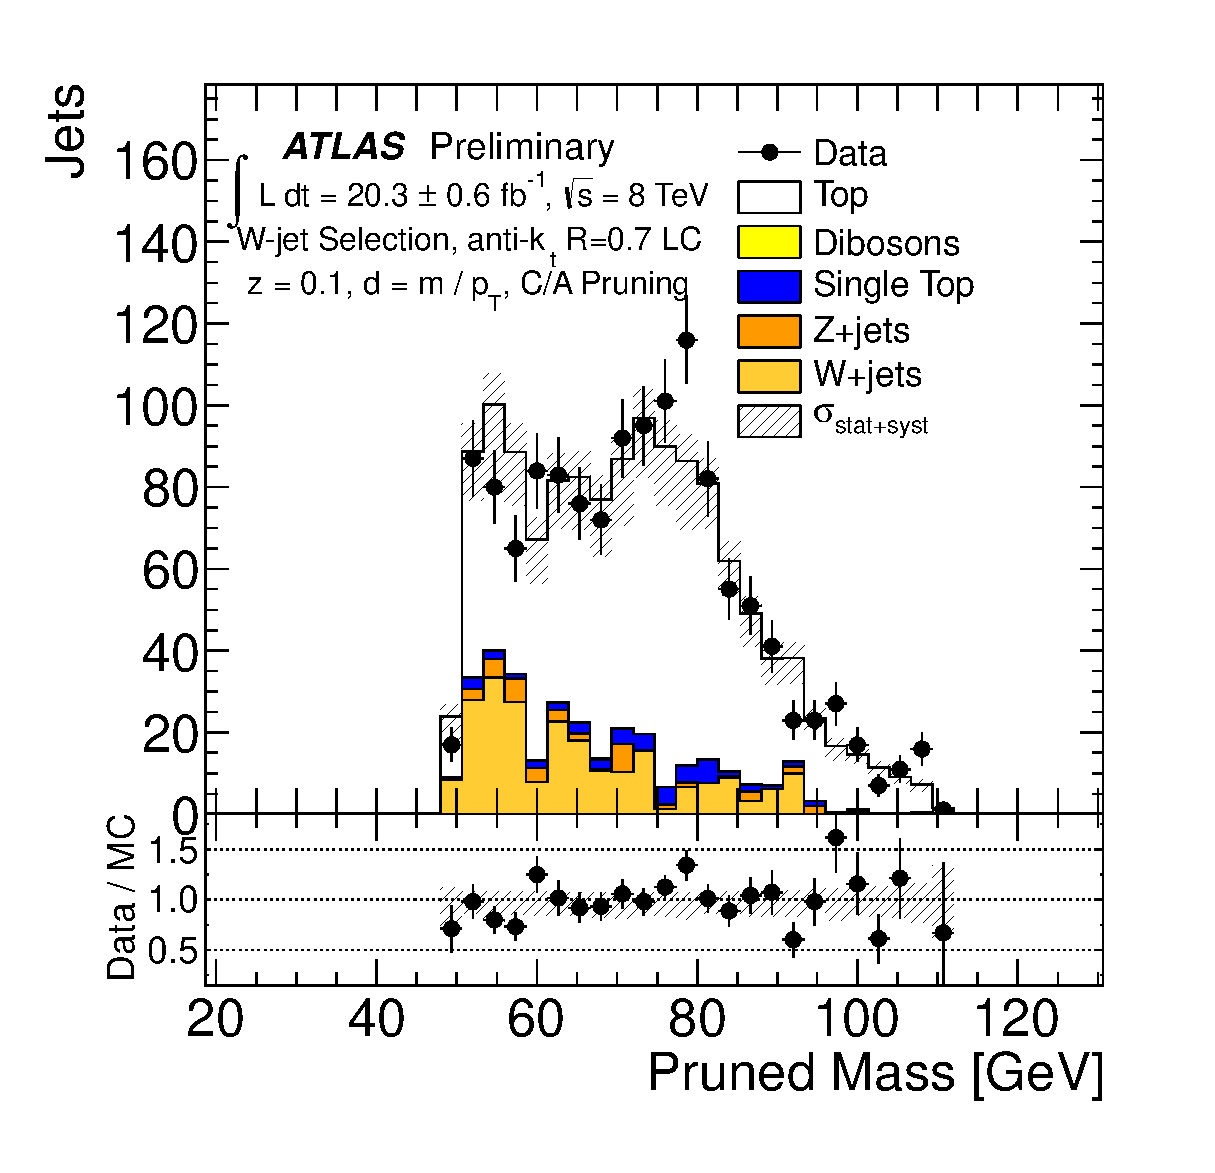
\includegraphics[width=.45\textwidth]{NoGroomedBOverlapWithMassCutAntiKt7LCTopoPrunedCamKtZCut10DCut50_lj_m_PT200_eta0_Top_WithData.eps}}
\subfigure[\label{fig:WpeakQCD}]{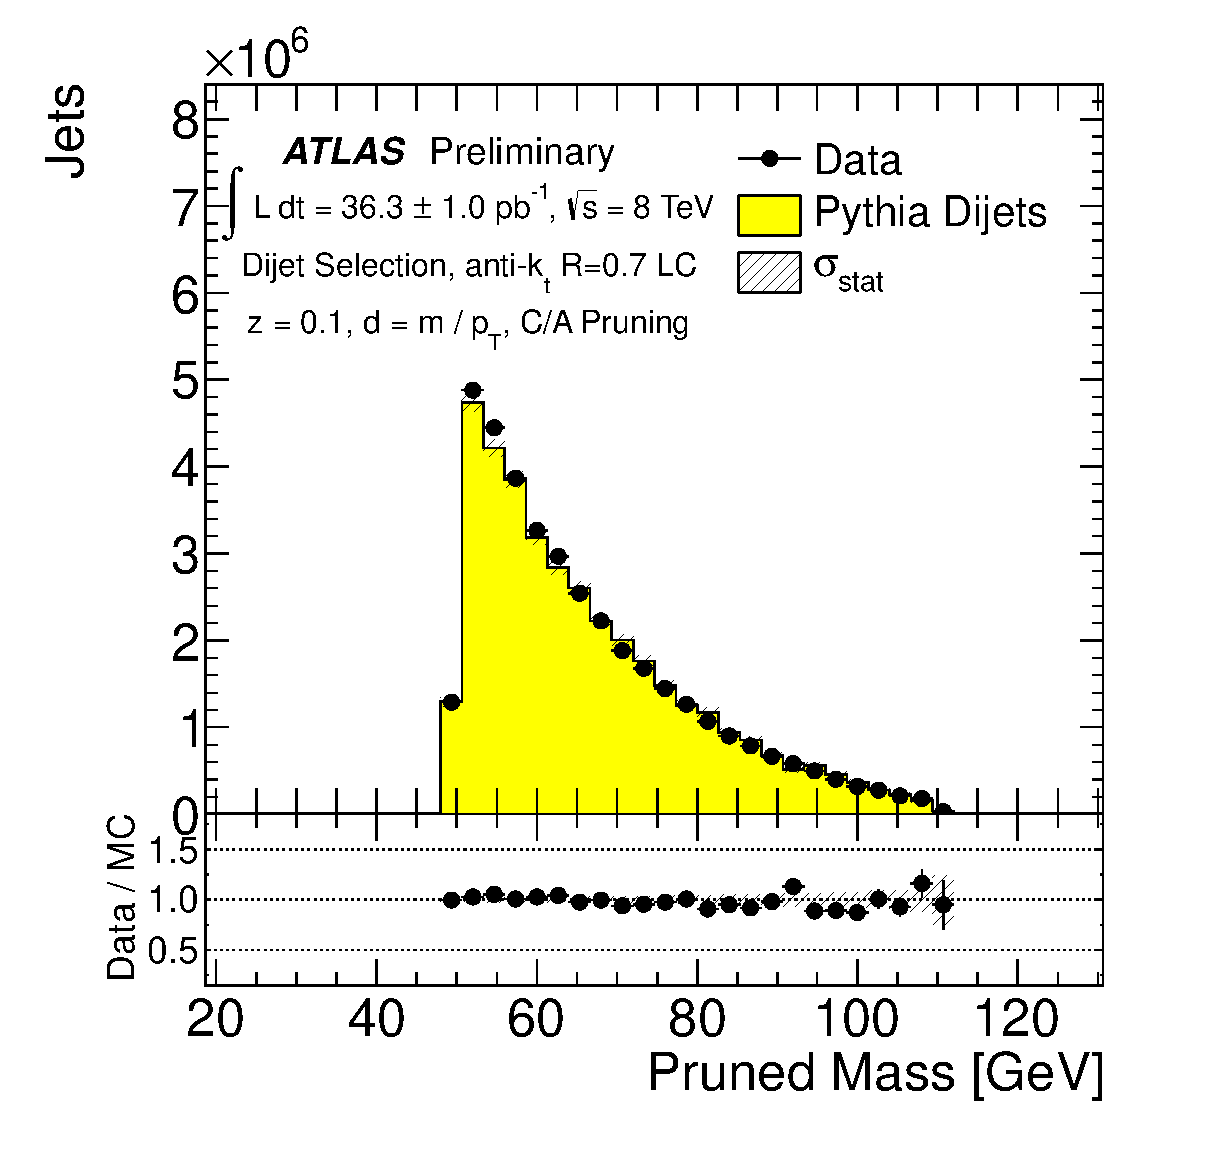
\includegraphics[width=.45\textwidth]{WithMassCutAntiKt7LCTopoPrunedCamKtZCut10DCut50_lj_m_PT200_eta0_WithData.eps}}
\caption{Pruned, leading jet mass distribution in data and in simulation for (a) a $W$-jet selection and for (b) a dijet selection. $W$-jet selection plots show statistical and systematic uncertainties whereas dijet selection plots show statistical uncertainties only.}
\label{fig:Wpeak}
\end{figure}

%----------------------------------------------------
% Background rejection
%----------------------------------------------------
\subsection{Signal efficiency and background rejection}
\label{app:qjets:jetvol:rejection}

As enriched samples of $W$-jets and dijets are selected in both data and MC, the combined light quark and gluon jet rejection as a function of $W$-jet efficiency can be measured separately in both data and MC. The $W$-jet efficiency and dijet rejection (the inverse of the dijet efficiency) are calculated by scanning cut values of the volatility distributions in Figure~\ref{fig:DataMC_vol}. The results in Figure~\ref{fig:SEvsBR} show that a rejection factor of 15 for a mixed sample of light quark and gluon jets can be obtained at a $50\%$ $W$-jet efficiency working point, and they also confirm that $\alpha = 0.1$ provides the optimal background rejection for a fixed signal efficiency as discussed in section~\ref{app:qjets:jetvol:alpha}. All samples are selected as described in Section~\ref{app:qjets:event-selection}. Figure~\ref{fig:SEvsBRMCback} shows the efficiency in MC and includes the backgrounds discussed in Section~\ref{app:qjets:datasets} while Figure~\ref{fig:SEvsBRdata} shows the efficiency in data and confirms the rejection observed in MC.

\begin{figure}[htbp]
\centering
%\subfigure[\label{fig:SEvsBRMC}]{\includegraphics[width=.45\textwidth]{NoGroomedBOverlapWithMassCutAntiKt7LCTopo_lj_MassVolatility_PT200_eta0Graph.eps}}
\subfigure[\label{fig:SEvsBRMCback}]{\includegraphics[width=.45\textwidth]{VvsAlphaGraphMC.eps}}
\subfigure[\label{fig:SEvsBRdata}]{\includegraphics[width=.45\textwidth]{VvsAlphaGraph.eps}}
\caption{Signal efficiency versus background rejection in (a) signal MC with all backgrounds and in (b) data for several values of $\alpha$.}%  {\bf [*** data plot to be updated when QCD finishes running]}}
\label{fig:SEvsBR}
\end{figure}

In Figure~\ref{fig:SEvsBRQ}, the signal efficiency to background rejection is computed for several values of $N_{QJets}$. Values of $N_{QJets} > 25$ show very similar results, suggesting that generation of as few as 25 Q-jets per jet can provide near optimal performance as discussed in section~\ref{app:qjets:jetvol:number}.

\begin{figure}[htbp]
\centering
\includegraphics[width=.45\textwidth]{VvsAlphaGraphMCN.eps}
\caption{Signal efficiency versus background rejection for several values of $N_{QJets}$. Performance stabilizes for $N_{QJets} > 25$.}%  {\bf [*** update with b overlap]}}
\label{fig:SEvsBRQ}
\end{figure}

%----------------------------------------------------
% Track jets
%----------------------------------------------------
\subsection{Track jets performance}
\label{app:qjets:jetvol:trackjets}

As a cross-check on the method, the studies are also performed using jets reconstructed from tracks in the inner detector while event selections are still performed on the $R=0.4$ calorimeter jets. As shown in Figure~\ref{fig:WQCDTrack}, some discrimination between $W$-jets and dijets continues to exist for jets constructed from tracks, but the separation is significantly reduced compared to the calorimeter variable. This is expected due to the missing neutral content, which varies widely from jet to jet due to the fragmentation of an individual jet, and consequently means that distributions for discriminating variables are generally less well separated. Figure~\ref{fig:DataMCTrack} shows the comparison of data and simulation as a function of volatility for the $W$-jet selection. %\textsl{\textbf{Ed.} These plots will be updated soon to fix the statistics issue-- problem is well understood.}

\begin{figure}[htbp]
\centering
%\subfigure[{\bf [***to be fixed]}\label{fig:SEvsBRMCTrack}]{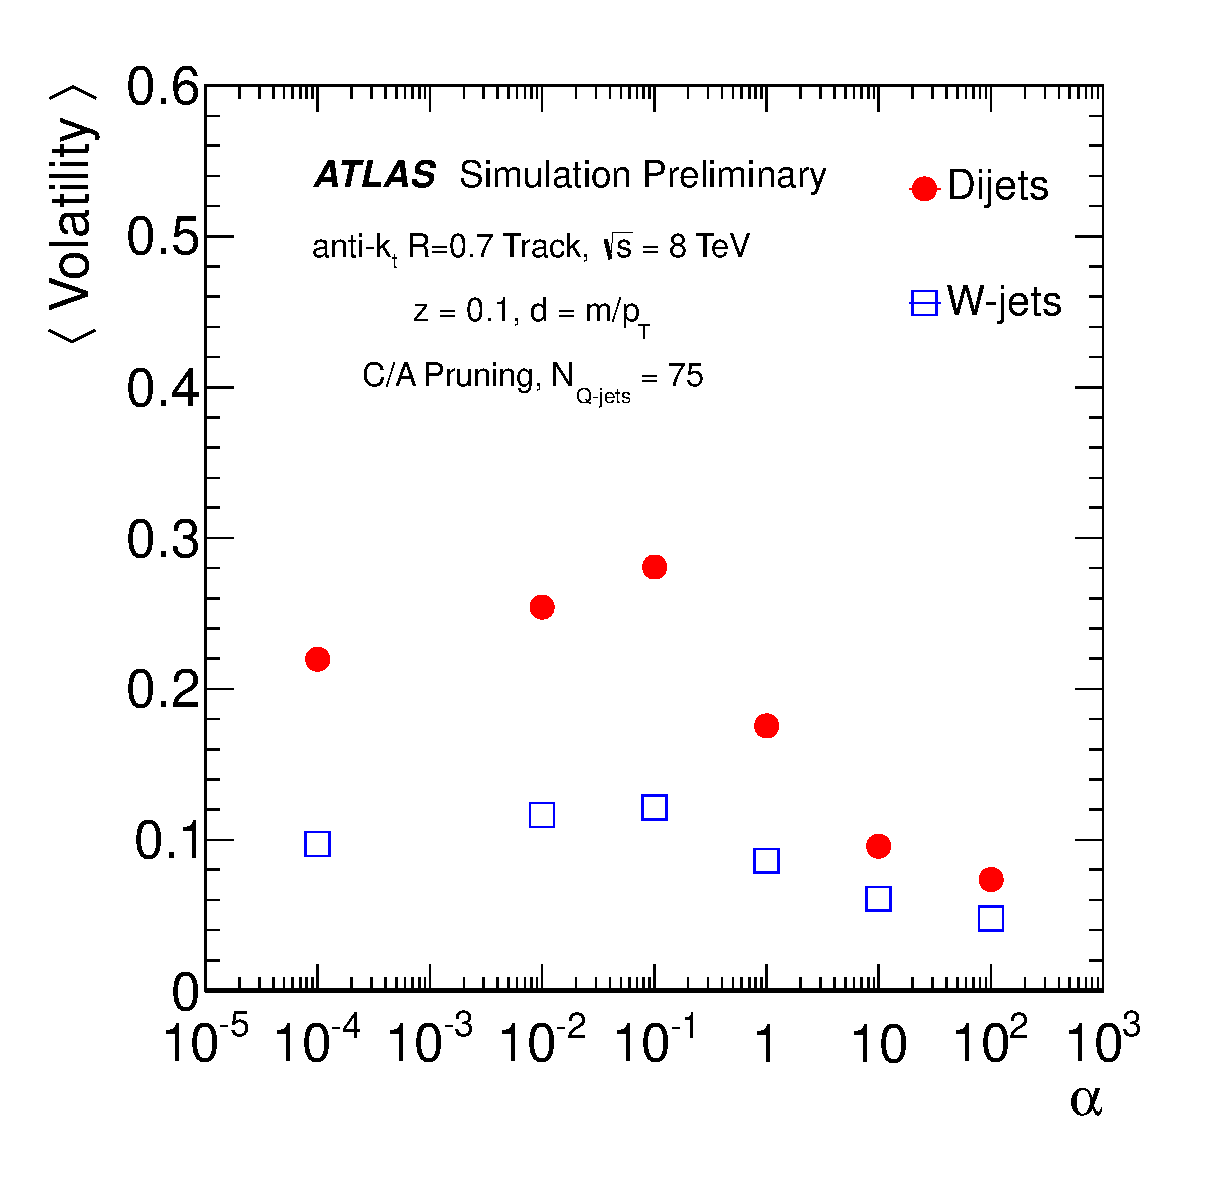
\includegraphics[width=.45\textwidth]{NoGroomedBOverlapAntiKt7TrackZ_lj_MassVolatility_PT200_eta0_mean.eps}}
\subfigure[\label{fig:WQCDTrack}]{\includegraphics[width=.45\textwidth]{NoGroomedBOverlapWithMassCutAntiKt7TrackZ_lj_MassVolatility_PT200_eta0Log.eps}}
\subfigure[\label{fig:DataMCTrack}]{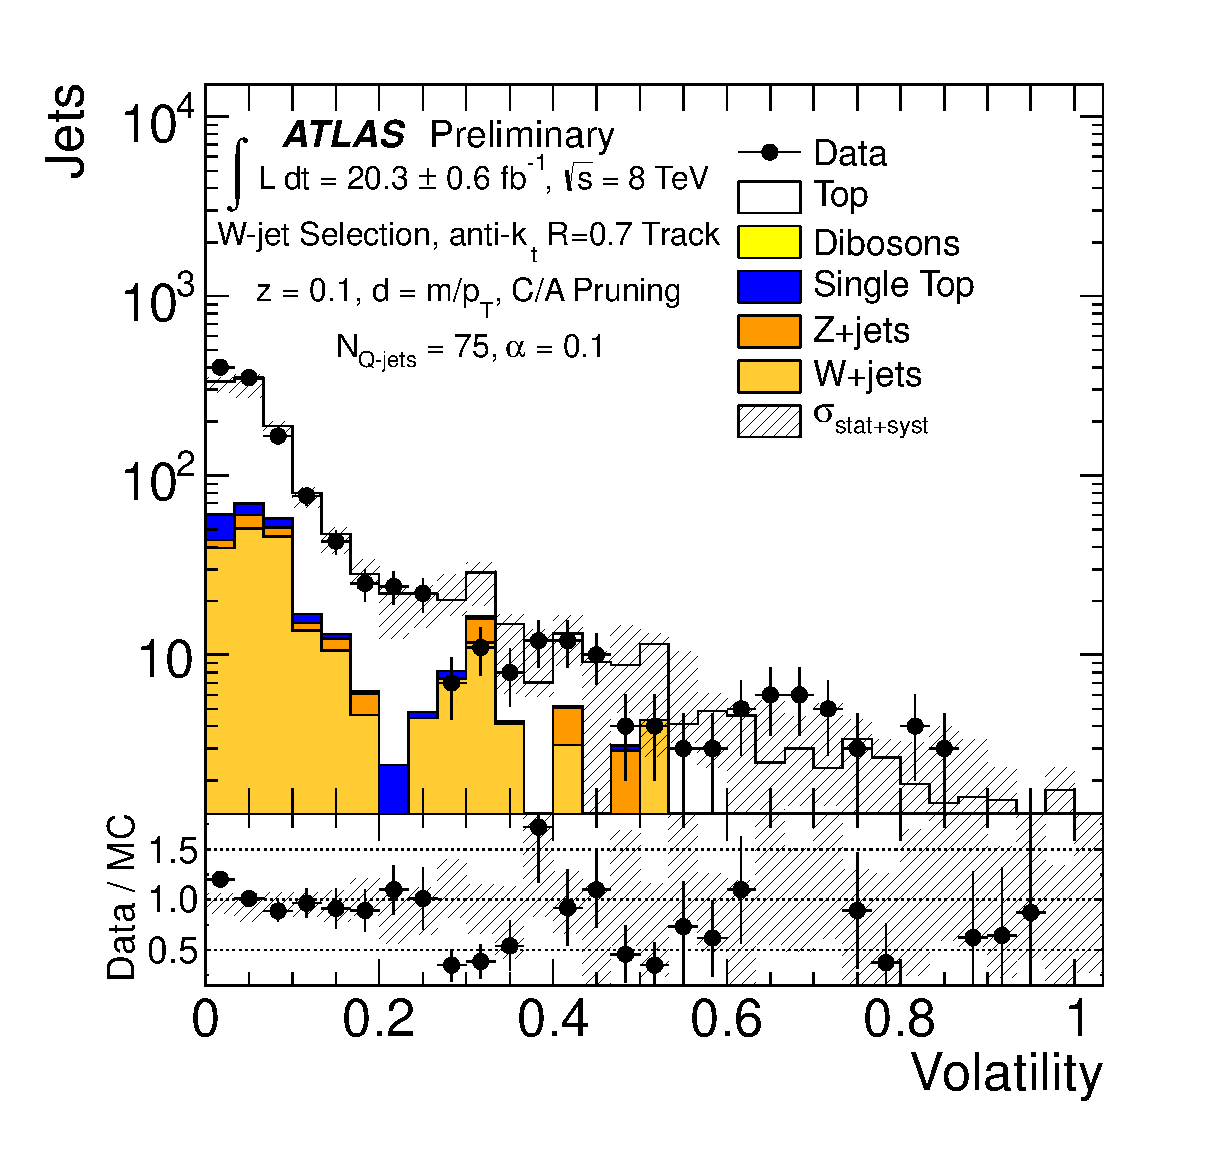
\includegraphics[width=.45\textwidth]{NoGroomedBOverlapWithMassCutAntiKt7TrackZ_z1_d5_emin0_emax0_rig1000_NJets75_lj_MassVolatility_PT200_eta0_WithData_Logy.eps}}
\caption{Volatility, constructed using track-jets, of $W$-jets and dijets (a) and data/MC agreement for the same in the $W$-jet selection (b). The separation is reduced compared to calculating the variable from calorimeter clusters.}
\label{fig:tracks}
\end{figure}

% Lynn: taken this out for now, stats really poor, why are they so drastically different to calo jets?
%\begin{figure}[htbp]
%\centering
%\subfigure[]{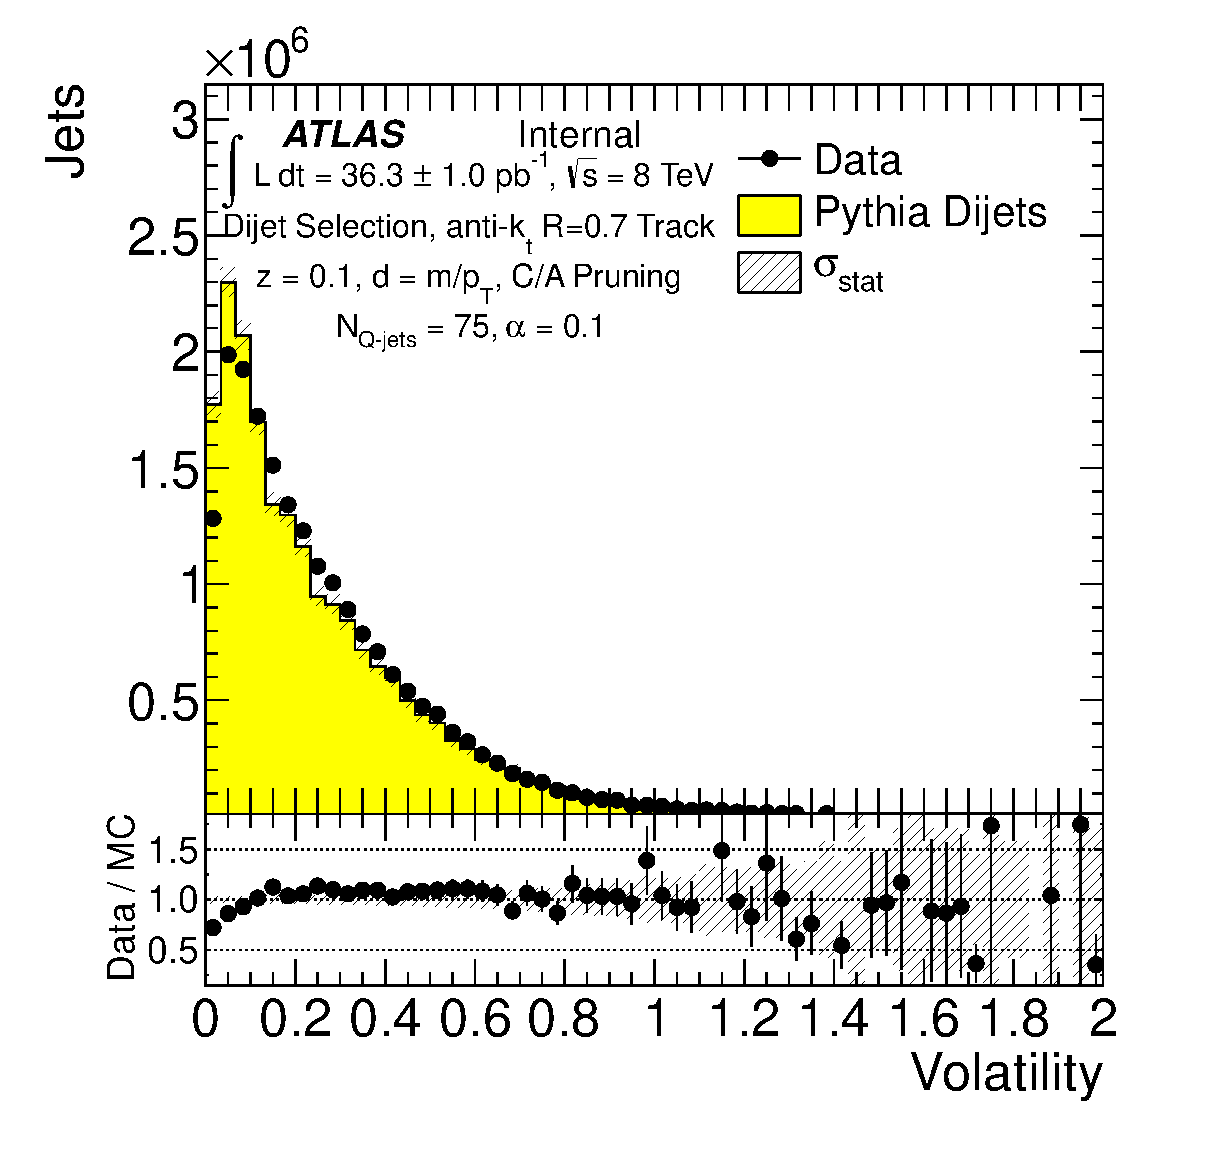
\includegraphics[width=.45\textwidth]{WithMassCutAntiKt7TrackZ_z1_d5_emin0_emax0_rig1000_NJets75_lj_MassVolatility_PT200_eta0_WithData.eps}}
%\subfigure[]{\includegraphics[width=.45\textwidth]{NoGroomedBOverlapWithMassCutAntiKt7TrackZ_z1_d5_emin0_emax0_rig1000_NJets75_lj_MassVolatility_PT200_eta0_WithData.eps}}
%\caption{Data/MC comparison.}
%\label{fig:DataMC_vol}
%\end{figure}

%----------------------------------------------------
% Q-jets vs nsubjettiness
%----------------------------------------------------
\subsection{Q-jets versus $N$-subjettiness performance}
\label{app:qjets:jetvol:nsubj}

To compare the volatility variable of the Q-jets algorithm to other substructure algorithms, the $\tau^{\rm min}_{21}$ $N$-subjettiness variable with one pass of the minimization algorithm on the $k_t$ axes has been chosen\footnote{Note that while the jet selections are performed using the pruned jet kinematics, $N$-subjettiness is calculated with the full jet constituents, consistent with the approach that has delivered best experimental performance in previous efforts~\cite{ATLAS:2012am}.}~\cite{nsub,Thaler:2011gf,ATLAS:2012am}. Figure~\ref{fig:VvsNsubGraph} shows that the performance of the two variables is comparable over a large range of signal efficiency and background rejection values. Figure~\ref{fig:vol_vs_tau21min} shows the correlations between the two variables with correlation factors of 50\% and 24\% for jets from a hadronically-decaying $W$ boson and dijets respectively. In particular, for the dijet selection shown in Figure~\ref{fig:vol_vs_tau21min_QCD}, the slope between the two variables is reduced for large volatility values. This confirms previous observations~\cite{MattHadroWorkshop} that a combination of the two variables will give an improved performance. 

\begin{figure}[htbp]
\centering
\subfigure{\includegraphics[width=.46\textwidth]{VvsNsubGraph.eps}}
\caption{Signal efficiency versus background rejection for the volatility and $\tau^{\rm min}_{21}$ variables.}
\label{fig:VvsNsubGraph}
\end{figure}

\begin{figure}[htbp]
\centering
\subfigure[\label{fig:vol_vs_tau21min_W}]{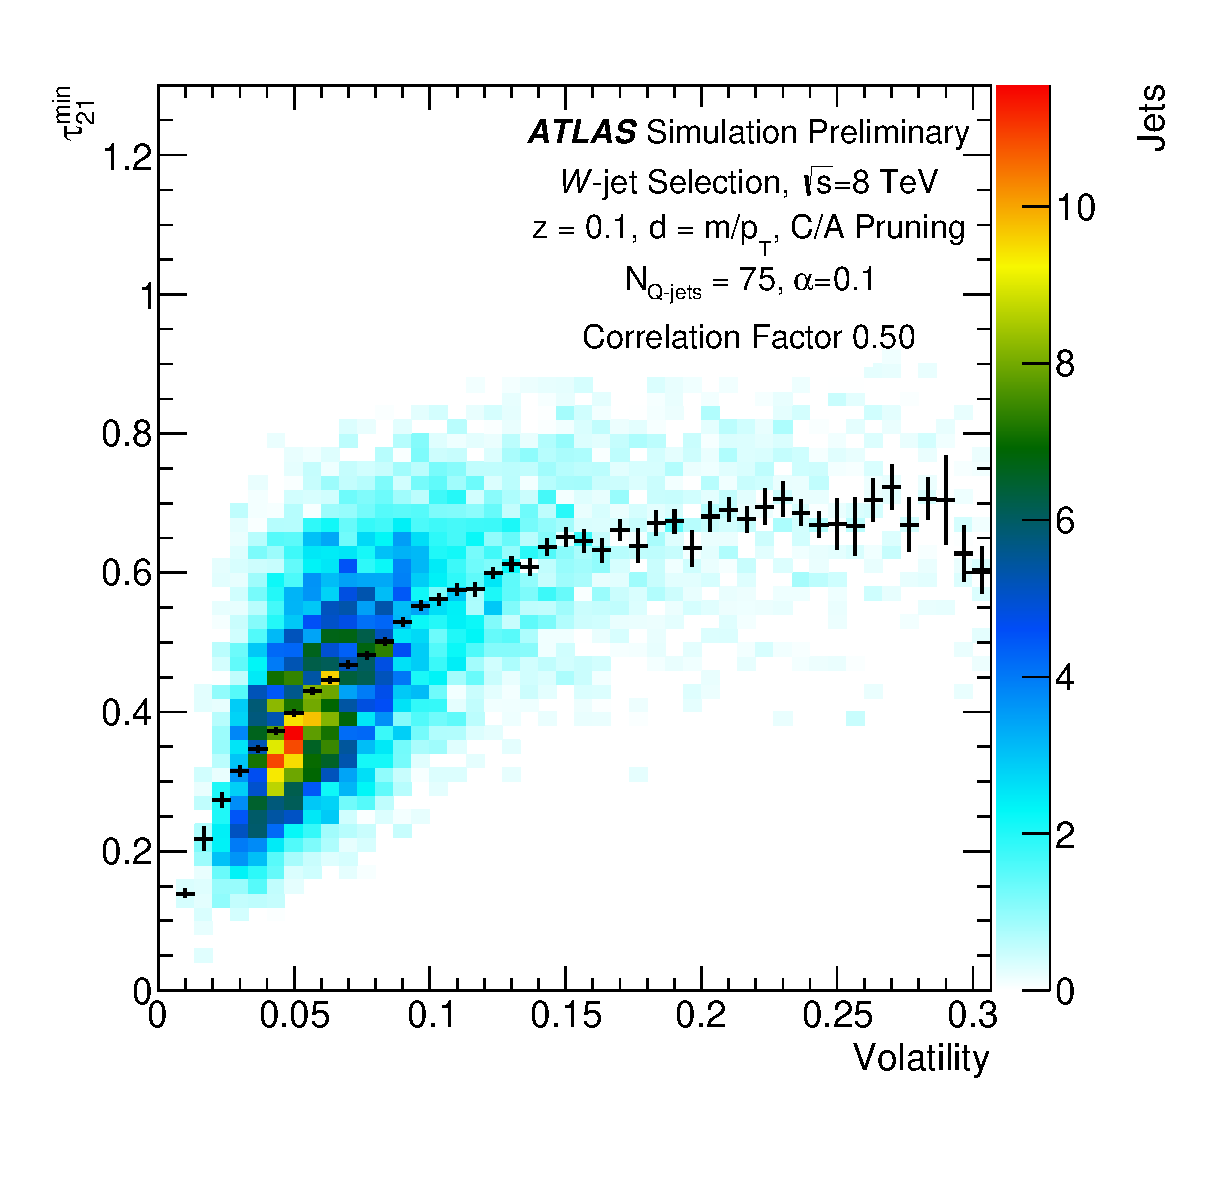
\includegraphics[width=.455\textwidth]{vol_vs_tau21min_W.eps}}
\subfigure[\label{fig:vol_vs_tau21min_QCD}]{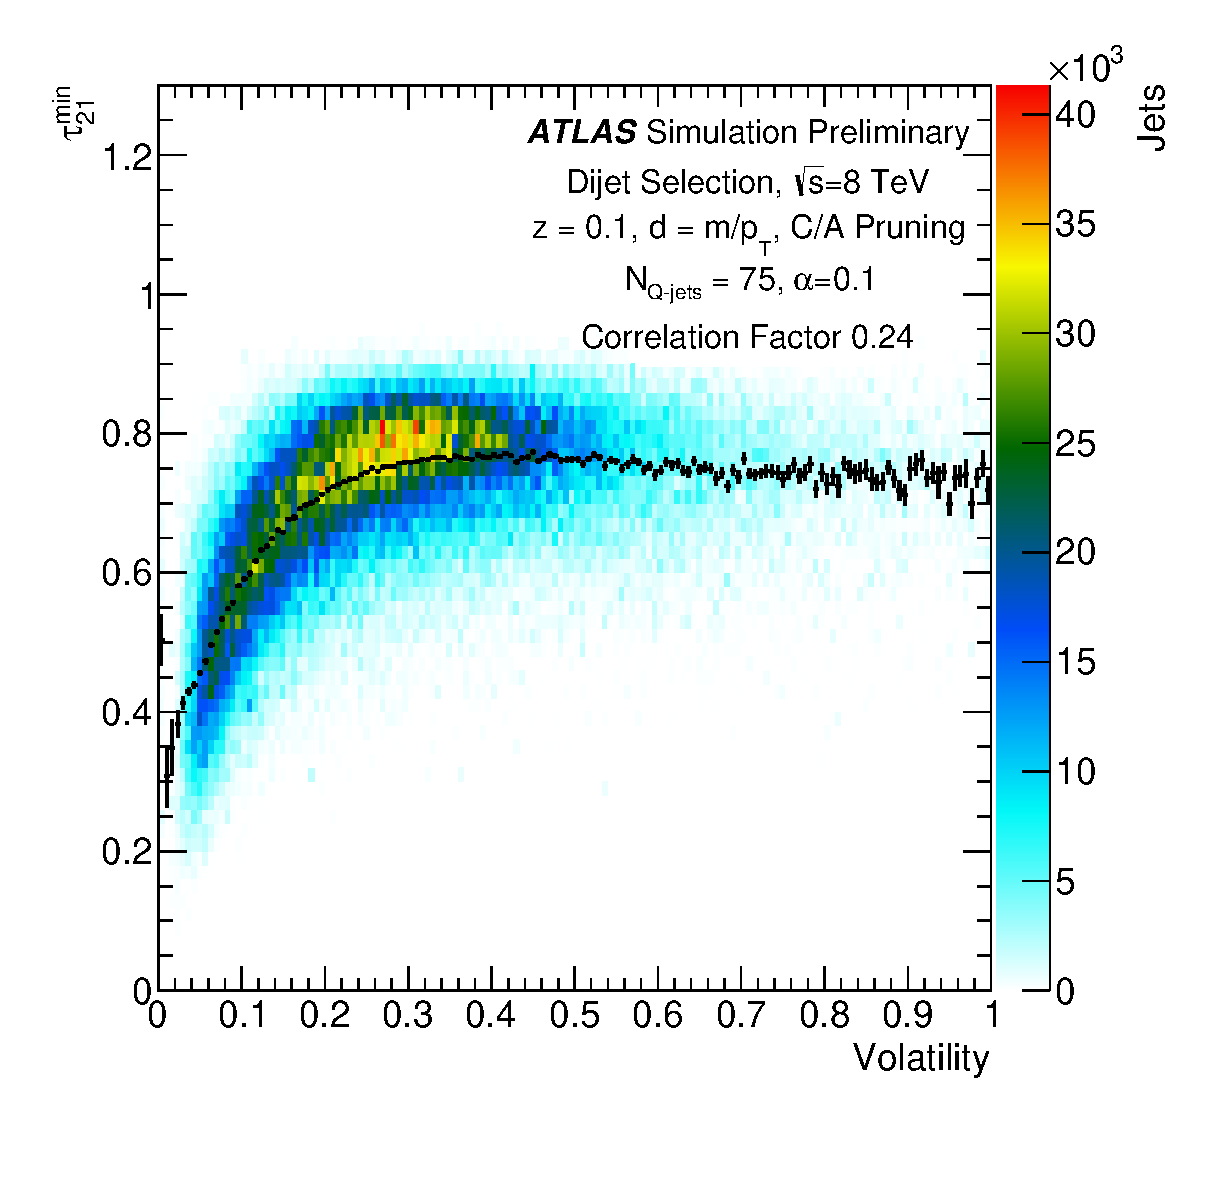
\includegraphics[width=.455\textwidth]{vol_vs_tau21min_QCD.eps}}
\caption{Distributions of the $\tau^{\rm min}_{21}$ ($N$-subjettiness) and volatility (Q-jets) variables for (a) a $W$-jet selection and (b) a dijet selection. The black points represent the mean $\tau^{\rm min}_{21}$ value as a function of volatility.}
\label{fig:vol_vs_tau21min}
\end{figure}

\section{Conclusions}

The performance of the Q-jets reclustering algorithm the jet volatility observable have been explored and this technique has been confirmed to discriminate between $W$-jets and light quark and gluon jets. Two free parameters of the algorithm have been studied and optimal values for the rigidity at $\alpha=0.1$ and for the number of Q-jets per jet of $N_{QJets}>25$ have been determined. No strong pile-up dependence is observed for the volatility variable, while the distribution for jets from a $W$ boson decay are slightly more sensitive to additional interactions than light quark and gluon jets. The performance of the Q-jet algorithm in terms of discrimination power between $W$-jets and light quark and gluon jets has been studied for jets reconstructed from topological calorimeter clusters and for jets reconstructed from inner detector tracks; the discrimination of the latter is seen to be weaker. This degradation in performance is partially due to the fact that neutral hadrons do not leave tracks in the inner detector. 

From these studies, the application of a volatility requirement is shown to give a factor of 15 in dijet rejection for $50\%$ $W$-jet efficiency for jets with $200$ GeV $< p_T < 350$ GeV. The separation is validated in-situ by comparing distributions of samples enriched in $W$-jets and light quark and gluon jets: very good agreement is observed in multijet events, and fairly good agreement is seen in $W$-jets. The separation power of Q-jets is also tested directly in data using these samples, and the Monte Carlo predictions are confirmed. Lastly, the signal efficiency and background rejection of the volatility variable has been shown to be similar to the $\tau^{\rm min}_{21}$ $N$-subjettiness variable, while the former performs slightly better in the high $W$-jet efficiency region. The correlations between these two variables have been studied and interesting regions of decorrelaton are observed, particularly for the dijet selection. This suggests that a combination of the two variables could lead to an improved performance. 

For some time, the Q-jets approach provided (along with n-subjettiness, in other regions of $W$-efficiency)the best approach to $W$ tagging at ATLAS. Recent developments~\cite{EEC} have displaced the effectiveness of this technique, but other useful characteristics remain. For example, creating an observable like volatility is just one tool provided by the $Q$-jets approach: one could also imagine treating cuts on events not as binary decisions, but as flexible weights calculated by measuring decisions over various $Q$-jet like reconstructions of the event~\cite{Ellis:2012sn}. Such approaches can significantly improve the statistical power of searches, but challenges remain in applying them to analyses\footnote{In particular, almost all statistical tools on the experiments assume integer-like statistics for data, and do not handle weighted data very well.}. Both ATLAS and CMS have only scratched the surface of this technique, and more interesting results are certainly possible.